%% main_zh.tex - NeurIPS 2026 中文版本
%% 编译命令：xelatex main_zh && bibtex main_zh && xelatex main_zh && xelatex main_zh

\documentclass{article}
\usepackage{neurips_2026}
\usepackage[UTF8,fontset=none]{ctex}
\setCJKmainfont{Songti SC}[BoldFont=Heiti SC]
\setCJKsansfont{Heiti SC}
\setCJKmonofont{Songti SC}

%% 核心数学
\usepackage{amsmath}
\usepackage{amssymb}
\usepackage{amsthm}
\usepackage{mathtools}

%% 表格
\usepackage{booktabs}
\usepackage{multirow}
\usepackage{array}
\usepackage{tabularx}

%% 图表
\usepackage{graphicx}
\usepackage{subcaption}
\graphicspath{{figures/}}

%% 颜色与超链接
\usepackage{xcolor}
\usepackage[colorlinks=true,linkcolor=blue!70!black,citecolor=blue!70!black,
            urlcolor=blue!70!black]{hyperref}

%% 引文
%% natbib 由 neurips_2026.sty 加载

%% 算法
\usepackage{algorithm}
\usepackage{algpseudocode}

%% 其他
\usepackage{microtype}
\usepackage{enumitem}
\usepackage{xspace}

%% ---- 自定义宏 ----
\newcommand{\reff}{\ensuremath{r_{\mathrm{eff}}}\xspace}
\newcommand{\SAk}{\ensuremath{\mathrm{SA}_k}\xspace}
\newcommand{\Ddir}{\ensuremath{\Delta_{\mathrm{dir}}}\xspace}
\newcommand{\Gr}{\ensuremath{\mathrm{Gr}(k,d)}\xspace}
\newcommand{\R}{\ensuremath{\mathbb{R}}}
\newcommand{\norm}[1]{\ensuremath{\left\lVert#1\right\rVert}}
\newcommand{\nucnorm}[1]{\ensuremath{\left\lVert#1\right\rVert_{*}}}
\newcommand{\ScoreC}{\ensuremath{\mathrm{Score}_C}\xspace}
\newcommand{\UID}{\ensuremath{\mathrm{UID}}\xspace}

%% ---- 定理环境 ----
\newtheorem{theorem}{定理}
\newtheorem{lemma}{引理}
\newtheorem{proposition}[lemma]{命题}
\newtheorem{corollary}[lemma]{推论}
\newtheorem{remark}{注释}
\newtheorem{definition}{定义}

%% ============================================================
\title{坍缩模型：基于谱几何的无标签数据池压缩}
\author{%
  匿名作者\\
  NeurIPS 2026 匿名提交%
}

\date{}

\begin{document}
\maketitle

% ============================================================
\begin{abstract}
给定 $M$ 候选数据集，哪个 $k{\ll}M$ 子集在特征合并后最好地保留了表示多样性——无需访问标签或下游任务？
我们通过推导 \textbf{坍缩模型} 来解决这一无标签的数据池压缩问题，该模型是一个由精确局部谱几何启发的结构化摘要预测器。该模型通过两个与压缩相关的 SVD 通道（能量比 $\gamma$、方向对齐 $\alpha$）从一个 $2{\times}2$ 格拉姆块特征值结构中预测合并的有效秩 ($\reff$)，从而生成基于模型的超加性诊断指标 $\rho_c(\alpha,\gamma)$，该指标驱动仅使用 \emph{每个数据集的摘要统计} 的贪婪压缩算法——适用于隐私受限或流式设置，在这些设置中无法共享特征。在来自 5 种编码器家族和 2 种模态的 427 对真实特征矩阵上，公式达到了皮尔逊 $r{=}0.97$。基于坍缩指导的压缩几乎是最优的（相对于完全搜索的 ${\leq}1\%$ 后悔），在保留方面与最近发表的谱多样性基线 (Vendi-Greedy) 相匹配，同时仅需要摘要统计而不是完整的特征矩阵，并且在下游线性探针准确性上优于设施位置 / $k$-质心（符号检验 $p{<}10^{-3}$，坍缩超过随机的 $95\%$ 置信区间）。比较揭示了两个不同的 LP 相关多样性轴（由坍缩捕获的谱保持率和由最远点遍历捕获的质心覆盖），澄清了何时每种信号占主导地位。该框架扩展到最多 $14{\times}$ 压缩比的 $M{=}43$ 数据池，并通过 CLIP 和 DINO 编码器中揭示出二态主角分布来识别监督 / 自监督谱几何学之间的定量分界线。代码可在 \url{https://anonymous.4open.science/r/collapsemodel-1DB6} 获取。
\end{abstract}
% ============================================================
\section{引言}
\label{sec:intro}

现代预训练模型越来越多地依赖于从多个候选数据集组合特征——多领域迁移学习、用于自监督预训练的数据整理 \citep{gadre2023datacomp} 和持续学习都面临同样的问题：
\emph{给定 $M$ 个候选数据集，哪些 $k{\ll}M$ 的子集在特征拼接后能保留完整池的多样性？}
我们称之为 \emph{无标签的数据池压缩} 问题：与经典的核心集选择 \citep{mirzasoleiman2020coresets} 和最近的 \emph{样本级} 数据整理方法（DSIR~\citep{xie2023dsir}, DsDm~\citep{engstrom2024dsdm}, D$^2$ 剪枝~\citep{maharana2023d2pruning}) 不同，我们寻求在 \emph{数据集级别} 的压缩（而非样本级别），且不依赖标签或下游任务。评判标准是表示多样性，形式化为合并特征的有效秩 $\reff(H)=\exp(-\sum_i p_i\log p_i)$ \citep{roy2007effective,garrido2023rankme}。此前没有研究描述数据集级别谱和相对子空间几何在特征拼接下如何共同影响有效秩，迫使实践者依赖于穷举搜索或扩展性差的启发式方法。

先前的研究解决了相关但不同的问题。
\emph{谱多样性度量} 如 RankMe~\citep{garrido2023rankme}, VNE~\citep{kim2023vne}, 和 Vendi 分数~\citep{friedman2023vendi,pasarkar2024cousins} 通过奇异值或相似矩阵谱的熵来量化单个集合的多样性；它们不预测两个集合在拼接下的多样性如何结合。
\emph{无标签核心集选择} (ELFS~\citep{shen2025elfs}, ZCore~\citep{griffin2024zcore}, DEFT-UCS~\citep{das2024deft}) 通过几何或代理动力学来选择样本子集；它与我们的数据集级别表述互补但不相关。
\emph{池级整理} (DataComp~\citep{gadre2023datacomp}, DataComp-LM~\citep{li2024dclm}, DsDm~\citep{engstrom2024dsdm}, Quad~\citep{zhang2025quad}) 使用过滤或模型感知启发式方法，但没有闭合形式的多样性准则。
\emph{表示相似性度量} (SVCCA \citep{raghu2017svcca}, PWCCA \citep{morcos2018pwcca}, CKA \citep{kornblith2019similarity}, PARC \citep{bolya2021parc}) 比较两个表示但不预测合并后的秩。
\emph{迁移性估计器} (LogME \citep{zhang2021logme}, H-分数 \citep{bao2019hscore}, TransRate \citep{huang2022transrate}, LEEP \citep{li2021nleep}, 重新评估由 \citet{ibrahim2022newer}) 和基于 PMI 的数据集估值~\citep{zhang2024pmi} 预测下游准确性但要么需要标签，要么不建模合并。
Task2Vec \citep{achille2019task2vec} 无需标签但需要探针微调。
模型合并方法 (任务算术~\citep{ilharco2023task}, TIES-合并~\citep{yadav2023ties}, DARE~\citep{yu2024dare}) 合并参数而非特征。
固有维数工作 \citep{pope2021intrinsic,ansuini2019intrinsic} 描述单个矩阵但不描述合并后的矩阵。
据我们所知，没有现有研究结合精确的局部谱分析 $\reff([H_A;H_B])$ 与数据集级别选择的汇总统计预测器。
我们从精确恒等式 $G_{A\cup B}=G_A+G_B$ 出发推导 \textbf{坍缩模型}。
在明确的成对方向条件下，引理~\ref{lem:gram} 使用逐模态能量比 $\gamma_i$ 和对齐度 $\alpha_i$ 给出精确的 $2\times2$ 块特征值；在比例谱和均匀对齐条件下，命题~\ref{prop:proportional} 给出精确的双分支熵公式。
对于一般谱，Eq.~\eqref{eq:pred} 将这种结构压缩为四个摘要——$r_A$、$r_B$、全局能量比 $\gamma$ 和 平均对齐度 $\alpha$，并且被明确地视为经验近似。
其诊断阈值 $\rho_c(\alpha,\gamma)$ 描述了三种理想化的行为模式：超加性、方向塌陷和能量塌陷。
我们的 $\SAk$ 使用主角线余弦的均方误差，这比 SVCCA 的无符号余弦或 PWCCA 的能量加权形式更直接地与投影理论相关；
$U$-channel 使用了 Two-NN 内在维度估计器 \citep{facco2017estimating}。
\begin{figure}[t]
\centering
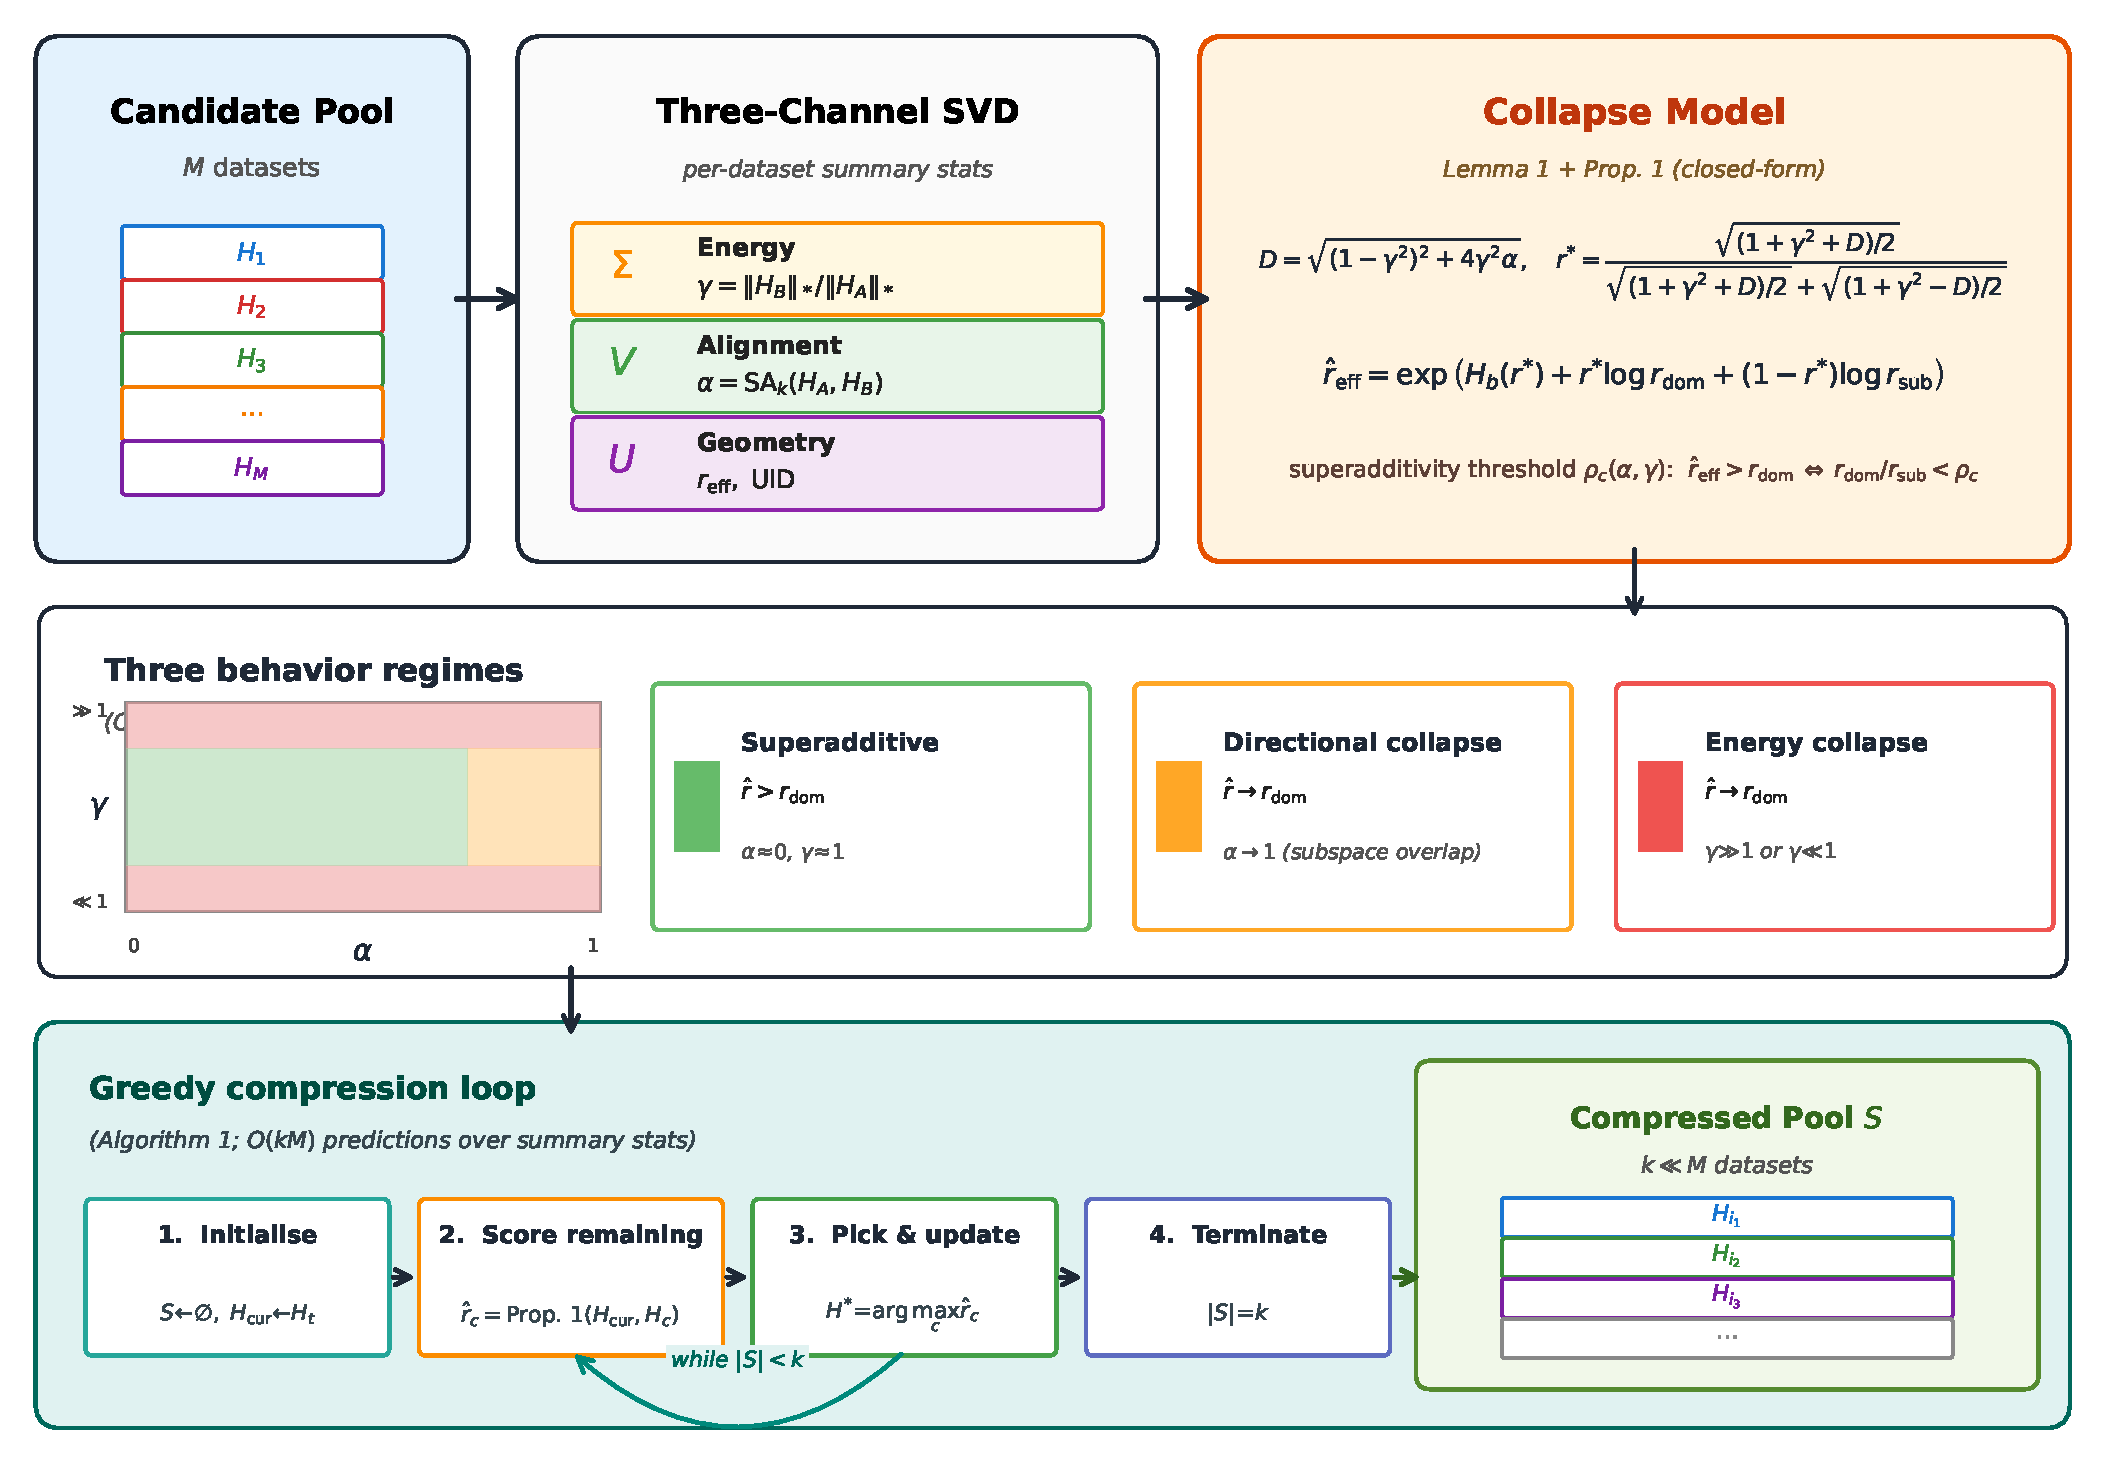
\includegraphics[width=0.88\linewidth]{fig_framework.pdf}
\caption{无标签数据池压缩流水线。
\textbf{顶部:} 每个数据集的摘要（$\Sigma{:}\gamma$, $V{:}\alpha$, $U{:}\reff$）将引理~\ref{lem:gram} 的确切模式结构压缩成近似预测器 Eq.~\eqref{eq:pred} 及其诊断阈值 $\rho_c(\alpha,\gamma)$。
\textbf{中部:} 在 $(\alpha,\gamma)$ 平面中的三种行为模式（定理~\ref{cor:superadd}）：超加性、方向塌陷 ($\alpha{\to}1$)、能量塌陷 ($\gamma{\gg}1$ 或 ${\ll}1$)。
\textbf{底部:} 贪心循环（算法~\ref{alg:collapse_greedy}）：评估剩余候选者，选择 $\arg\max$，重复 $k$ 次；输出压缩池 $S$。}
\label{fig:framework}
\end{figure}
\textbf{为什么基于摘要的压缩？}
在 $M$ 个候选者中进行穷举搜索需要 $\binom{M}{k}$ 个合并的 SVD，每个为 $O(Nd^2)$，同时访问所有特征矩阵（$M=14, k=5$: $2002$ 个 SVD；$M=100, k=10$: $1.7 \times 10^{13}$）。崩溃模型将此减少为从每个数据集的摘要统计中得出的 $O(kM)$ 秩预测，从而在隐私受限和流式设置中实现压缩。

\textbf{贡献。}
(1)~\emph{问题表述}---\emph{无标签的数据池压缩}（Sec.~\ref{sec:compression}）：一个 $\mathcal{O}(kM)$ 的贪婪算法，基于每个数据集的摘要统计（$\reff,\|\cdot\|_*,V_{\mathrm{top}\text{-}k}$），适用于特征矩阵不能共享的隐私受限和流式设置。
(2)~\emph{精确局部理论与结构化近似}（Proposition~\ref{prop:gram_general}, Lemma~\ref{lem:gram}, Proposition~\ref{prop:proportional}）：无条件的 Gram 表示、精确的成对方向特征值分解以及比例谱熵公式。对于一般谱，我们推导出一个低维摘要预测器，并通过反例证明其四个输入不足以进行通用精确预测。
(3)~\emph{LP相关多样性的两信号分解}（Sec.~\ref{sec:compression}）：与现代基线的基准测试表明，下游相关的多样性可以分解为两个正交信号---\emph{谱保持率}（由崩溃模型捕获，$r_A+r_B$，Vendi-Greedy）和 \emph{质心覆盖}（由最远点遍历捕获）。两阶段的 Cen$\to$Col 混合体组合了这两个信号，并在 $k=10$ 时同时在 LP 和保持率上优于纯崩溃模型（Appendix~\ref{app:p2e_hybrid}），将结构化公式定位为可组合的基本构建块而非独立策略。
\textbf{实证发现。}
公式在 280 组受控 + 120 组非主角点 + 427 组真实配对样本上进行了验证，这些样本来自 5 种编码器家族和 2 种模态（Pearson $r{=}0.97$, $R^2_{\mathrm{cal}}{=}0.95$）。
该框架识别出监督/自监督光谱几何学的定量分界：ResNet-50 在 91 组配对样本上实现了 $100\%$ 超加性效应，而 CLIP 和 DINO 只在跨域合并中达到了 $29$--$36\%$ 的水平——这一差距通过模型隔离出的二模态主角点分布机制得到了机械解释。

在无标签分析中，只有塌缩模型同时提供了基于摘要的合并秩预测（$R^2_{\mathrm{cal}}{=}0.95$ 在 427 组配对样本上，表~\ref{tab:e1d}），行为模式诊断通过 $\rho_c(\alpha,\gamma)$ 和相同 $O(Nd\min(N,d))$ 成本下的超加性效应诊断；朴素的 $r_A{+}r_B$ 在序数排名上与塌缩模型匹配（$\rho{=}0.963$ vs.\ $0.966$，无显著差异），但缺乏绝对 $R^2$、行为模式诊断和冗余检测。

% ============================================================
\section{背景：SVD 三通道分解}
\label{sec:background}

对于任何特征矩阵 $H\in\R^{N\times d}$，其薄奇异值分解为 $H=U\Sigma V^\top$（$U\in\R^{N\times r}$, $\Sigma=\mathrm{diag}(\sigma_1\geq\cdots\geq\sigma_r>0)$,
$V\in\R^{d\times r}$），该分解分离出三种正交的表示方面。

\textbf{$\Sigma$ 通道 --- 谱能量。}
\textbf{有效秩} 总结了谱分布：
\begin{equation}
  \reff(H) = \exp\!\left(-\sum_{i=1}^r p_i \log p_i\right),
  \quad p_i = \frac{\sigma_i}{\sum_j \sigma_j},
  \label{eq:reff}
\end{equation}
其中 $p_i$ 是奇异值份额（未平方），因此 $r_{\mathrm{eff}}\in[1,r]$。
核范数 $\|H\|_*=\sum_i\sigma_i$ 捕捉总能量。
定义在附录~\ref{app:proof_prop1} 中的谱差数量（谱转移缺口）在那里被用作 Gram 块转移界线的一部分。
\textbf{$V$ 通道 --- 方向结构。}
右奇异向量 $V$ 编码了哪些方向被激活。
\begin{definition}[子空间对齐度]
\label{def:sa}
令 $\hat{V}_A^k,\hat{V}_B^k\in\R^{d\times k}$ 是 $H_A,H_B$ 的前 $k$ 个右奇异向量。
在级别 $k$ 的 \textbf{子空间对齐度} 定义为：
\begin{equation}
  \SAk(H_A,H_B) = \frac{1}{k}\norm{\hat{V}_A^{k\top}\hat{V}_B^k}_F^2
  = \frac{1}{k}\sum_{i=1}^k\cos^2\theta_i,
  \label{eq:sak}
\end{equation}
其中 $\theta_1\leq\cdots\leq\theta_k$ 是主角度。
\end{definition}
$\SAk\in[0,1]$: $\SAk=0$ 表示完美正交子空间（最大互补性）；
$\SAk=1$ 表示相同子空间（合并后没有新方向）。

\textbf{$U$ 通道 --- 样本几何。}
左奇异向量 $U\in\R^{N\times r}$ 编码了样本的几何分布。
通过最近邻估计的 \textbf{U 空间固有维度 (\UID)}:
\begin{equation}
  \mathrm{UID}(H) = \frac{1}{\log 2\cdot\mathbb{E}[\log(\mu_2/\mu_1)]},
  \label{eq:uid}
\end{equation}
其中 $\mu_1,\mu_2$ 是单位球体 $S^{k-1}$ 上最近邻和次近邻的测地线距离（L2 正则化后的 $U_k$ 行）。

\textbf{每个通道的作用。}
$\gamma$ 和 $\alpha$ 进入合并秩预测公式
(第 \ref{sec:method} 节) 并驱动压缩算法。
\UID 描述了单个数据集的内在几何结构
并在编码器诊断 (第 \ref{sec:e1d} 节) 中使用，但
并不出现在预测公式中；它在此处包括以完成表示空间的正交分解。

\textbf{独立性。}
成对 Spearman 检验（Bonferroni 校正，$n{=}15$ 个探针）在 ResNet-50 或
ViT-B/16 上检测到三个通道之间没有显著相关性 (所有 $p_{\mathrm{Bonf}}{>}0.38$)，这与
$\gamma,\alpha,\UID$ 捕捉了不同的属性一致。
% ============================================================
\section{塌陷模型}
\label{sec:method}

\subsection{设置与符号表示}
\label{sec:setup}

令 $H_A\in\R^{N_A\times d}$ 和 $H_B\in\R^{N_B\times d}$ 为 L2 行归一化的特征矩阵，其有效秩分别为 $r_A=\reff(H_A)$, $r_B=\reff(H_B)$，核范数分别为 $\|H_A\|_*$, $\|H_B\|_*$，子空间对齐度为 $\alpha=\SAk(H_A,H_B)$。定义：
\begin{equation}
  \gamma = \frac{\|H_B\|_*}{\|H_A\|_*} \in (0,\infty),
  \quad
  r_{\mathrm{dom}} = \begin{cases}r_A & \gamma\leq1 \\ r_B & \gamma>1\end{cases},
  \quad
  r_{\mathrm{sub}} = \begin{cases}r_B & \gamma\leq1 \\ r_A & \gamma>1\end{cases}.
\end{equation}
$\gamma$ 是这两个矩阵的 \textbf{能量比}；$r_{\mathrm{dom}}$ 是高能矩阵的有效秩。

\subsection{主要结果}
\label{sec:theorem}

我们的分析分离了三个不能混淆的层次：无条件的格朗日恒等式、在显式解耦假设下的精确成对方向模型以及一般谱的低维摘要预测器。

\begin{proposition}[精确的格朗日表示]
\label{prop:gram_general}
令 $H_A=U_A\Sigma_A V_A^\top$ 和
$H_B=U_B\Sigma_B V_B^\top$ 为紧奇异值分解，将 $V_A$ 完成到一个正交基 $Q_A=[V_A\;V_{A,\perp}]$。用
$C=Q_A^\top V_B$ 和 $\widetilde\Sigma_A^2$ 表示 $\Sigma_A^2$ 填充零以达到维度 $d$，合并的格朗日算子满足
\begin{equation}
 Q_A^\top(H_A^\top H_A+H_B^\top H_B)Q_A
 =\widetilde\Sigma_A^2+C\Sigma_B^2C^\top.
 \label{eq:general_gram}
\end{equation}
因此，合并的奇异值是右侧特征值的平方根。
\end{proposition}

方程~\eqref{eq:general_gram} 是无条件的。一般情况下 $C$ 是稠密的：一个矩阵的一个奇异方向可以耦合到另一个矩阵的多个方向。单独的谱和平均主角统计量因此不能决定合并后的谱。
\begin{lemma}[Exact: 2$\times$2 Gram Block Eigenstructure]
\label{lem:gram}
假设成对且解耦的方向：对于每个 $i$，$V_{B,i}=\cos\theta_i V_{A,i}+\sin\theta_i V_{\perp,i}$，其中两个二维平面 $\mathrm{span}\{V_{A,i},V_{\perp,i}\}$ 互为正交。定义 \emph{模式-wise} 能量比 $\gamma_i=\sigma_{B,i}/\sigma_{A,i}$ 和 $\alpha_i=\cos^2\theta_i$。第 $i$ 个 Gram 块的特征值
\begin{equation}
 \lambda_{\pm,i}=\frac{\sigma_{A,i}^2}{2}
 \left(A_i\pm D_i\right),\quad
 A_i=1+\gamma_i^2,\quad
 D_i=\sqrt{(1-\gamma_i^2)^2+4\gamma_i^2\alpha_i}.
  \label{eq:discriminant}
\end{equation}
对应的奇异值为 $\sqrt{\lambda_{+,i}}$ 和 $\sqrt{\lambda_{-,i}}$。在所述配对和解耦条件下，此结果是精确的（附录~\ref{app:proof_thm})。
\end{lemma}

全局比值 $\gamma=\|H_B\|_*/\|H_A\|_*$ 并不意味着 $\gamma_i=\gamma$。用集合 $\{\gamma_i,\alpha_i\}$ 替换为全局摘要 $(\gamma,\alpha)$ 是一个近似步骤。

\begin{proposition}[精确比例谱模型]
\label{prop:proportional}
在引理~\ref{lem:gram} 下，进一步假设对于每个 $i$ 有 $\sigma_{B,i}=\gamma\sigma_{A,i}$ 和 $\alpha_i=\alpha$。令 $A=1+\gamma^2$, $D=\sqrt{(1-\gamma^2)^2+4\gamma^2\alpha}$，并
\begin{equation}
 q = \frac{\sqrt{(A+D)/2}}
 {\sqrt{(A+D)/2}+\sqrt{(A-D)/2}}.
  \label{eq:rstar}
\end{equation}
则合并谱由 $H_A$ 的两个缩放副本组成，并且
\begin{equation}
 r_{\mathrm{merged}}=r_A\exp(H_b(q)),\qquad r_A=r_B.
 \label{eq:proportional_exact}
\end{equation}
\end{proposition}

\begin{definition}[塌陷摘要预测器]
\label{def:collapse}
对于一般谱，我们将模式-wise 量压缩为全局核范比 $\gamma$ 和平均最高 $k$ 对齐度 $\alpha$，计算 $q$ 来自式~\eqref{eq:rstar}，并定义
\begin{equation}
  \hat{r}_{\mathrm{merged}} =
  \exp\!\Big(H_b(q) + q\log r_{\mathrm{dom}} + (1-q)\log r_{\mathrm{sub}}\Big),
  \label{eq:pred}
\end{equation}
其中 $H_b(p)=-p\log p-(1-p)\log(1-p)$。
\end{definition}
Equation~\eqref{eq:pred} 是一个基于理论的低维近似，而不是恒等式或普遍有界的估计器。它插值输入谱熵并加上理想化的两分支分裂的二元熵。其在一般谱上的准确性是一个经验问题，在 Sec.~\ref{sec:experiments} 中评估。

\textbf{解释。}
Equation~\eqref{eq:pred} 是个体秩加权对数几何平均值加上一个平衡奖金 $H_b(q)$（当 $q{=}0.5$ 时最大，随着 $q{\to}0,1$ 而消失）。

\textbf{行为模式。}
\emph{超加性} ($\alpha{\approx}0$, $\gamma{\approx}1$): $q{\approx}0.5$, $\hat{r}_{\mathrm{merged}}{\approx}2\sqrt{r_Ar_B}\geq r_{\mathrm{dom}}$。
\emph{方向塌陷} ($\alpha{\to}1$): $q{\to}1$, $H_b(q){\to}0$, $\hat{r}_{\mathrm{merged}}{\to}r_{\mathrm{dom}}$。
\emph{能量塌陷} ($\gamma{\gg}1$ 或 $\gamma{\ll}1$): $q{\to}1$, $\hat{r}_{\mathrm{merged}}{\to}r_{\mathrm{dom}}$。
当 $\alpha{\to}1$ \emph{和} $\gamma{\gg}1$ 时，合并的秩可以 \emph{低于} $r_{\mathrm{sub}}$——净损失多样性。

\subsection{超加性阈值}
\label{sec:superadd}

\begin{corollary}[摘要-模型超加性诊断]
\label{cor:superadd}
Equation~\eqref{eq:pred} 中的摘要预测器在 $q<1$ 时预测
$\hat{r}_{\mathrm{merged}}>r_{\mathrm{dom}}$
当且仅当
\begin{equation}
  \frac{r_{\mathrm{dom}}}{r_{\mathrm{sub}}} < \rho_c(\alpha,\gamma)
  \;\equiv\; \exp\!\!\left(\frac{H_b(q)}{1-q}\right),
  \label{eq:rho_c}
\end{equation}
其中 $q$ 来自 Equation~\eqref{eq:rstar}。
阈值 $\rho_c$ 随 $\alpha$ 增加：$\rho_c\geq4.0$ 对所有 $\alpha\in[0,0.9]$ 在 $\gamma=1$ 时成立。
随着 $q\to1^{-}$，$\rho_c\to\infty$ 而预测的增益趋于零。
在退化点 $q=1$ 中，Equation~\eqref{eq:rho_c} 的除法未定义且 Equation~\eqref{eq:pred} 给出
$\hat r_{\mathrm{merged}}=r_{\mathrm{dom}}$ 精确值。
\end{corollary}
This is an exact decision boundary for the summary model, and for the proportional-spectrum model of Proposition~\ref{prop:proportional}; on general data it is a diagnostic rather than a guarantee.

\textbf{物理意义。}
$\rho_c$ 是摘要模型内部的一个决策阈值。在 $q=1$ 附近，它可以将任意小的正熵增量分类为超加性；因此 $\hat r_{\mathrm{merged}}-r_{\mathrm{dom}}$ 的大小必须与二元诊断一起报告。完全的方向重叠给出 $q=1$ 并无预测增益。证明和模型范围在附录~\ref{app:proof_thm}、\ref{app:pa_scope} 中。

\subsection{四份摘要不足以解决问题}
\label{sec:insufficiency}

\begin{proposition}[从四个标量无法唯一确定]
\label{prop:insufficient}
元组 $(r_A,r_B,\gamma,\alpha)$ 不能唯一确定 $\reff([H_A;H_B])$。
\end{proposition}

\textbf{反例。}
假设两个输入的奇异值均为 $(1,1)$，因此 $r_A=r_B=2$ 和 $\gamma=1$，并且在 $V_A=(e_1,e_2)$ 中有 $\R^4$。
对于对 X 取 $V_B=(e_1,e_3)$，给出每模式对齐 $(1,0)$。
对于对 Y 取
$V_B=((e_1+e_3)/\sqrt2,(e_2+e_4)/\sqrt2)$，给出对齐
$(1/2,1/2)$。两对都有相同的平均对齐 $\alpha=1/2$。
对 X 有合并奇异值 $(\sqrt2,1,1)$ 和有效秩
$2.958$，而对 Y 有两个副本的
$\sqrt{1+1/\sqrt2}$ 和 $\sqrt{1-1/\sqrt2}$ 并且有效秩 $3.661$。
因此相同的单个秩、全局能量比和平均对齐可以导致不同的合并秩。预测器必然丢弃对齐异质性、谱配对和跨方向耦合。
\hfill$\square$

\textbf{校准。}
在评估的真实数据对中，公式系统地高估了结果；单一的乘法常数 $c$ 恢复了定量准确性，并遵循了编码器家族间的通用回归 $c{=}0.946{-}0.175\log(N/\reff)$（附录~\ref{app:calibration}）。
由于这是一个在可观测变量 $\log(N/\reff)$ 上的一维线性模型，可靠估计 $c$ 只需每个编码器家族 $5$--$10$ 个带标签的样本对——这与计算冻结编码特征的成本相比是一个可以忽略不计的附加开销。在隐私受限的环境中，即使只有一个参考对的摘要统计信息可用，也可以估计每个编码器的 $c$ 而不会暴露任何原始特征。
同样的三个通道也界定了线性探针迁移损失（附录~\ref{app:proof_prop1}）：低 $\SAk$ 同时意味着 \emph{高} 合并增益和 \emph{高} 迁移损失。
% ============================================================
\section{摘要预测器的评估}
\label{sec:experiments}

在将坍缩模型应用于压缩（Sec.~\ref{sec:applications}）之前，我们建立了一个三步评估链：
(i) \textbf{理想化模型一致性}——预测器与其摘要假设下的数据一致 (§\ref{sec:e1a_main}，合成网格);
(ii) \textbf{真实数据的预测有效性}——公式在5种编码器家族、14个视觉数据集和19个文本语料库中仍然是一个强大的近似（§\ref{sec:e1d}，共427对）;
(iii) \textbf{行为模式一致性}——经验上的超加性模式与Corollary~\ref{cor:superadd}预测的三种模式一致 (§\ref{sec:e1d}，表~\ref{tab:e1d})。
这些测试共同验证了近似在何处成功、它如何转移到真实编码器以及其定性的诊断是否可观察。额外的控制（E1a-Ind 120个非主角对，E1b 30个真实对，E1c 57个对，E\_diverse跨架构，E\_downstream $\reff$/LP-准确性）均与同一图景一致，并在附录~\ref{app:exp_extras}中补充说明。
特征矩阵进行L2行归一化并子采样到$N_{\mathrm{sub}}$样本；有效秩使用公式~\eqref{eq:reff}；Bootstrap置信区间使用$B=10{,}000$次抽样。

\subsection{步骤 1 --- 理想化模型一致性：合成控制网格 (E1a, 280对)}
\label{sec:e1a_main}

在验证真实数据之前，我们在比例谱、成对方向模型下生成的280个受控合成对上验证了坍缩模型（$\alpha\in\{0,0.05,\ldots,1.0\}$和$\gamma\in\{0.1,0.33,\ldots,10.0\}$，$d{=}512$，$N{=}1000$，每种设置重复5次）。

\begin{table}[t]
\centering
\caption{E1a: 合成网格结果 ($N=280$)。朴素基线在大$\gamma$时失效。}
\label{tab:e1a}
\begin{tabular}{lcccc}
\toprule
方法 & $R^2$ & 最大误差 & 超加性 (\%) & $\alpha<1$ 超加性 \\
\midrule
朴素 $\sqrt{1+\alpha\gamma^2}$ & 0.30 & 28.73 & --- & --- \\
\textbf{坍缩模型 (我们的)} & \textbf{0.9999} & \textbf{0.27} & \textbf{87.5\%} & \textbf{100\%} (245/245) \\
\bottomrule
\end{tabular}
\end{table}
表~\ref{tab:e1a} 显示 $R^2{=}0.9999$（朴素基线为 $0.30$）。
在 $\alpha{<}1$ 的 245 种配置中，超加性比例均为 100\%；全部 35 个非超加性样例只出现在 $\alpha{=}1$（子空间相同）处，验证了推论~\ref{cor:superadd} 的退化边界。
$(\alpha,\gamma)$ 热图和超加性区域的可视化见附录~\ref{app:exp_extras}。

\subsection{步骤 2--3：真实数据泛化与行为区间一致性（E1d，427 对）}
\label{sec:e1d}

接下来，我们验证该公式能否推广到其合成推导范围之外，以及它所预测的三种行为区间能否在实验中观察到。
评估覆盖 5 个编码器家族（ResNet-50、ViT-B/16、CLIP ViT-B/32、DINO ViT-S/16、SBERT）、14 个视觉数据集（CIFAR-10/100、STL-10、SVHN、MNIST、Fashion-MNIST、BloodMNIST、DermaMNIST、PathMNIST，以及 5 个 ImageNet 语义子集 \emph{animal/vehicle/artifact/food/scene}）和 19 个 SBERT 文本语料库。
总计 \textbf{427 对}（ResNet-50 为 91 对，ViT-B/16、CLIP 和 DINO 各 55 对，SBERT 为 171 对）。

\begin{table}[h]
\centering
\caption{E1d：坍缩模型的大规模验证（427 对，5 个探针）。按编码器家族设置校准常数 $c$ 可恢复定量精度。}
\label{tab:e1d}
\small
\setlength{\tabcolsep}{3.5pt}
\begin{tabular}{lccccc}
\toprule
Probe & $n$ & Superadd.\  \% & Pearson $r$ & $c$ & $R^2_{\mathrm{cal}}$ \\
\midrule
ResNet-50 (14 datasets)       & 91  & \textbf{100\%}   & 0.940 & 0.776 & 0.760 \\
ViT-B/16 (11 datasets)        & 55  & 69.1\%            & 0.898 & 0.647 & 0.487 \\
CLIP ViT-B/32 (11 datasets)    & 55  & 29.1\%            & 0.950 & 0.595 & 0.839 \\
DINO ViT-S/16 (11 datasets)    & 55  & 36.4\%            & 0.913 & 0.584 & 0.554 \\
\midrule
\textbf{Vision (all probes)}   & \textbf{256} & \textbf{64.5\%} & \textbf{0.965} & \emph{per-probe} & \textbf{0.942} \\
+ SBERT text (19 corpora)      & +171 (427)   & 78.2\%           & 0.970          & \emph{per-probe} & 0.952 \\
\bottomrule
\end{tabular}\normalsize
\end{table}
\textbf{泛化（步骤 2）。}
该公式在全部 427 对真实数据上仍是较强的近似：未校准的总体 Pearson $r{=}0.970$，按编码器家族校准后 $R^2_{\mathrm{cal}}{=}0.952$（散点图见附录~\ref{app:exp_extras} 的图~\ref{fig:hero_scatter}）。
这表明，由理想化成对方向模型启发的摘要预测在监督 CNN、ViT、对比学习/自蒸馏 Transformer 和句子编码器等真实编码器上仍具有预测能力。

\textbf{行为区间一致性（步骤 3）。}
(i)~\textbf{ResNet-50 在 91 对数据上达到 100\% 超加性}（包括医学数据和 ImageNet），验证了推论~\ref{cor:superadd} 所预测的平衡 $(\gamma,\alpha)$ 区间。
(ii)~模型的方向重叠区间呈现出\textbf{监督/自监督分界}：CLIP 和 DINO 的超加性比例仅为 29\%--36\%，失败样例\emph{全部}集中在跨域数据对中（手写$\times$ImageNet、自然图像$\times$数字均失败），而域内数据对几乎全部成功。
其根本原因是双峰主角分布与极端条件数 $\kappa{\in}[10^4,10^6]$ 的共同作用（图~\ref{fig:bimodal_structure}），对应第~\ref{sec:superadd} 节的\emph{方向塌陷}区间。

\begin{figure}[t]
\centering
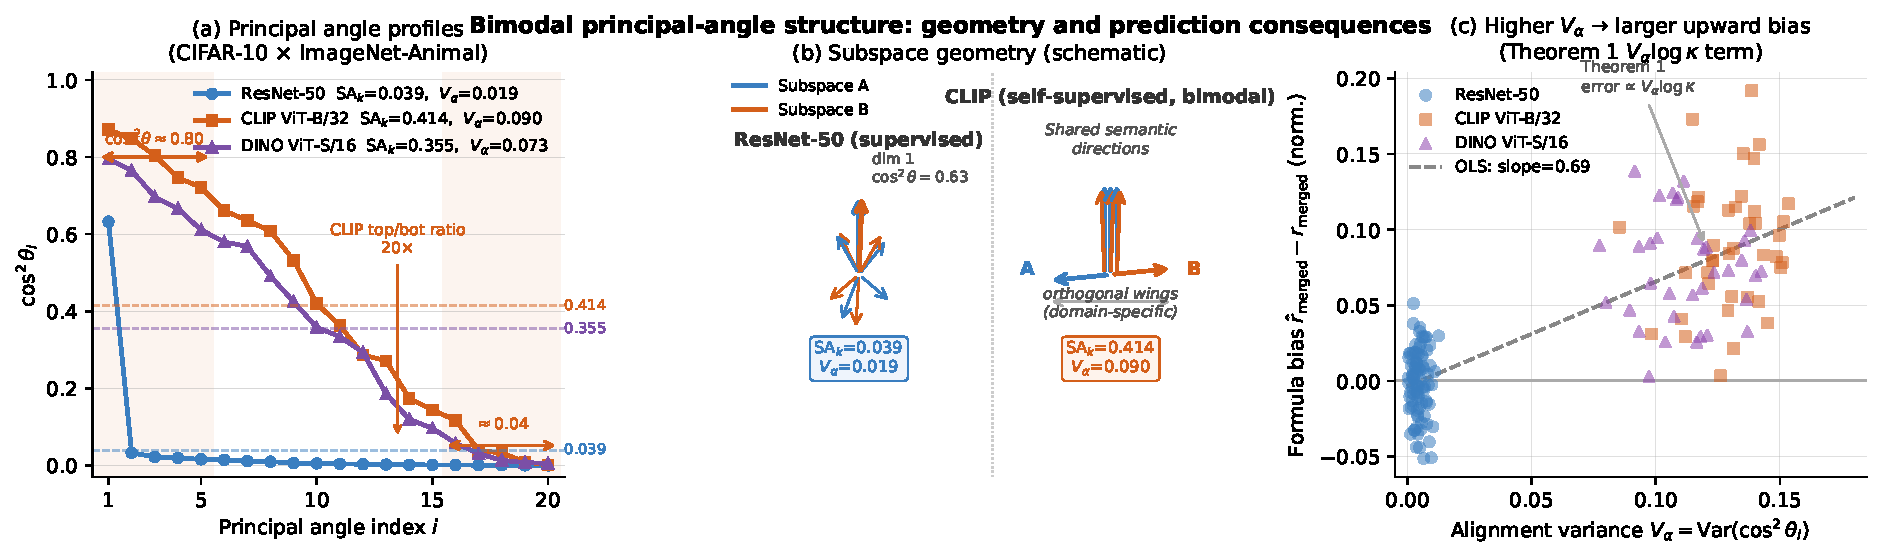
\includegraphics[width=0.97\linewidth]{fig_bimodal_structure.pdf}
\caption{\textbf{Bimodal principal-angle structure} (CIFAR-10\,$\times$\,ImageNet-Animal, $k{=}20$).
\textbf{(a)}~Per-dimension $\cos^2\theta_i$: ResNet-50 ($\SAk{=}0.039$, $V_\alpha{=}0.019$) decays monotonically from one dominant direction; CLIP ($\SAk{=}0.414$, $V_\alpha{=}0.090$) and DINO ($\SAk{=}0.355$, $V_\alpha{=}0.073$) form a two-cluster step (top-5 ratios $20{\times}$/$31{\times}$ over bot-5), violating the uniform-$\alpha$ assumption.
\textbf{(b)}~Geometric interpretation: one shared spine plus orthogonal domain-specific wings.
\textbf{(c)}~Alignment variance $V_\alpha$ predicts upward formula bias across 166 pairs (OLS slope 0.69), identifying alignment heterogeneity as an empirical failure indicator.}
\label{fig:bimodal_structure}
\end{figure}
\paragraph{量化双模态差距。}
每个探针校准后的 $R^2$: CLIP $0.84>$ ResNet $0.76>$ DINO $0.55>$ ViT $0.49$;
排名准确性普遍很高 ($r \geq 0.90$)。
Figure~\ref{fig:bimodal_structure}(a,c) 显示了 CLIP/DINO 的双聚类 $\cos^2\theta_i$ 分布 ($V_\alpha > 0.07$)，放大了观察到的预测偏差，识别出与全局摘要近似相比的具体偏离而非黑盒失败（完整机制见附录~\ref{app:bimodal})。

(iii) \textbf{能量塌陷} 出现在 ViT 的 17 对非超加性成对方向中，所有这些都在 $\gamma \notin [0.5,2]$ 中，与摘要模型的能量不平衡诊断一致。
(iv) \textbf{跨模态迁移}: 171 SBERT 文本成对方向 (98.8\% 超加性，排名 $r = 0.793$) 确认了公式的 \emph{序数} 预测是模态无关的。然而，绝对校准需要针对特定模态进行调整：视觉通用回归 ($c = 0.946 - 0.175\log(N/\reff)$, 附录~\ref{app:calibration}) 解释了 $R^2 = 0.96$ 的视觉方差，但仅解释了 $R^2 = 0.08$ 的 SBERT 方差，表明文本编码器具有质上不同的谱偏置。针对文本的校准留待未来工作。

\textbf{评估总结。}
步骤 1--3 确立了理想化模型的一致性、真实编码器上的强大经验排名以及可观察到的定性模式。它们并未确立普遍精确性：Proposition~\ref{prop:insufficient} 证明了四个摘要无法在一般情况下确定合并排名。
跨数据集校准泛化、跨探针一致性及 $\reff$/LP-准确率对应关系 ($\rho = 0.90$ 在 ViT 家族内) 见附录~\ref{app:exp_extras}。

% ============================================================
\section{从公式到应用：无标签数据池压缩}
\label{sec:applications}
\label{sec:compression}
\label{sec:pool_selection}

在评估了预测器（Sec.~\ref{sec:experiments}）之后，我们现在考察其实际用途：
给定 $M$ 个候选数据集和目标 $D_t$，将池压缩至 $k{\ll}M$ 的规模同时保持合并表示的有效秩 $\reff$。
穷举搜索 $\binom{M}{k}$ 子集是不可行的；
崩塌模型允许通过每个数据集的摘要统计信息进行 $O(kM)$ 预测来实现压缩。
每一轮，\textbf{BFG} 为每个剩余候选者评分，通过将 Eq.~\eqref{eq:pred} 应用于 $(H_{\mathrm{cur}},H_{\mathrm{cand}})$ 并选择预测出的最高 $\reff$（Algorithm~\ref{alg:collapse_greedy}）。
我们报告了两种证据水平：
(a) 在 $M{=}43$ 的 \emph{缩放压力测试} 中，该方法在异构规模下仍然有效（Table~\ref{tab:scale}），以及
(b) 与现代无标签基线的比较（Table~\ref{tab:p1a_modern}）；跨架构跨模态结果在 $M{=}14$ 的视觉池和 $M{=}7$ 的文本池中见 Appendix~\ref{app:compression_m14}。

每一轮，BFG 通过将 Eq.~\eqref{eq:pred} 应用于 $(H_{\mathrm{cur}},H_c)$ 来为每个剩余候选者评分——仅需从每个数据集的 SVD 中计算出 $\SAk$ 和 $\gamma$ ——并选择预测出的最高 $\reff$（附录~\ref{app:algorithm} 中有伪代码）。
基线：\textbf{Max-$\reff$}（最高的单一 $\reff$，忽略 $\alpha$）；
\textbf{$\Ddir$-贪婪}（通过 $\Ddir=1-\SAk$ 最大正交性，忽略 $\gamma$）；
\textbf{随机选择}（10 个均匀子集）。
在目标条件下的 $M{=}10$ 池中（ResNet-50 特征于 CIFAR-10/100、STL-10、SVHN、MNIST、Fashion-MNIST、BloodMNIST、DermaMNIST、PathMNIST 和 Oxford-Pets），预算 $K{\in}\{1,2,3,5\}$ 下，
\textbf{BFG 在 $K{\leq}3$ 时实现 $0\%$ 的后悔率，并在 $K{=}5$ 时实现 $1.0\%$ 的后悔率}——与穷举搜索相比，速度提高了三倍。
Max-$\reff$ 的召回率为 $67\%$；$\Ddir$-贪婪的后悔率为 $13\%$ 到 $20\%$。
所有策略在下游 LP 准确度上产生相同的结果，%
\footnote{LP 和 $k$-NN 排名高度相关：在 11 个探针 ${\times}$ 5 个数据集（共 53 对）中，
Spearman $\rho(\mathrm{LP},\mathrm{kNN\text{-}5}){=}0.980$
($p{<}10^{-33}$)。
我们报告了 LP；见附录~\ref{app:e7_knn} 了解 $k$-NN 的详细信息。}
这证实了最大化 $\reff$ 转化为下游可区分性（Appendix~\ref{app:e5_downstream}）。
\paragraph{大规模压缩。}
方向引导压缩在所有测试的设置中均保留了超过 $100\%$ 的完整池多样性——这一普遍现象是因为 $\reff$ 并非随池大小单调变化：添加冗余数据集会将归一化谱推向其模式并 \emph{减少} 熵，因此通过 $\alpha$ 通道去除冗余性会产生比完整池 \emph{更高} 的多样性压缩池。在 $M=14$ 视觉池中，Collapse 超过了 Facility Location ($+7$--$14$\,pp) 和 $k$-Medoids ($+8$--$14$\,pp)；在 $M=7$ 文本池（BERT/RoBERTa/GPT-2）中，它保留了 $103$--$106\%$ 的多样性（完整表格见附录~\ref{app:compression_m14})。在干净的精心整理的池中，当 $\bar\alpha<0.2$ 时，$r_A+r_B$ 和 Max-$\reff$ 算法与 Collapse 在 $M=43$ 时仅相差 $0.7$\,pp（表~\ref{tab:scale}）——这是由推论~\ref{cor:superadd} 预期的结果。在这样的池中，Collapse 模型的作用是提供一个 \emph{先验} 低冗余性诊断 ($\rho_c>4$ 在 $\bar\alpha\leq0.2$) 并在该条件失效时接管（克隆攻击、细粒度子集家族、双模态跨域对）；见附录~\ref{app:rsum_regime}。在 $k=7$ 的 $M=14$ 池中，Collapse Greedy 在几秒内运行，而 $\binom{14}{7}=3432$ 个耗尽合并 SVD 则需要更多时间。

\paragraph{$M=43$ 大规模压缩：压力测试。}
为了验证压缩优势在精心整理的池之外仍然成立，我们收集了 43 个 ResNet-50 数据集，覆盖 5 个 ImageNet 粗分类域、19 个 ImageNet 细粒度类别、10 个 MedMNIST 临床数据集和 9 个经典基准，并扫掠 $k\in\{3,5,7,10,14,20\}$（压缩比从 $14.3{\times}$ 到 $2.1{\times}$）。表~\ref{tab:scale} 报告了结果。

\begin{table}[h]
\centering
\caption{大规模压力测试 ($M=43$ ResNet-50; $M=11$ ViT-B/16)。
\textbf{Ret.}: $\reff^{\mathrm{sel}}/\reff^{\mathrm{full}}$ (\%)。
\textbf{LP}: 子空间投影线性探针准确率，5 个目标，10 次随机种子的平均值$\pm$标准差（§\ref{sec:applications})。FacLoc/kMedoids 被省略 ($O(M^2)$ 成本在此规模下)。}
\label{tab:scale}
\small
\setlength{\tabcolsep}{3.5pt}
\begin{tabular}{lcrrrcccc}
\toprule
& & \multicolumn{3}{c}{保留 (\%)} & \multicolumn{4}{c}{公平 LP 准确率} \\
\cmidrule(lr){3-5}\cmidrule(lr){6-9}
探针 & $k$ (比) & Collapse & Max-$\reff$ & Random & Collapse & Max-$\reff$ & Random & $\Delta$LP \\
\midrule
\multirow{4}{*}{ResNet-50} & 3 ($14.3{\times}$) & \textbf{112.4} & 112.4 & $71.0_{\pm15.5}$ & \textbf{0.7550} & 0.7550 & $0.7477_{\pm0.0050}$ & \textbf{$+0.0073$} \\
& 5 ($8.0{\times}$)  & \textbf{117.2} & 117.2 & $78.1_{\pm20.1}$ & \textbf{0.7560} & 0.7558 & $0.7502_{\pm0.0063}$ & \textbf{$+0.0058$} \\
& 7 ($5.7{\times}$)  & \textbf{117.4} & 117.4 & $80.5_{\pm15.1}$ & \textbf{0.7572} & 0.7572 & $0.7522_{\pm0.0048}$ & \textbf{$+0.0050$} \\
& 10 ($4.0{\times}$) & \textbf{116.2} & 116.2 & $90.8_{\pm7.5}$  & 0.7564 & 0.7564 & $0.7575_{\pm0.0024}$ & $-0.0011$ \\
\midrule
\multirow{3}{*}{ViT-B/16} & 3 ($3.7{\times}$) & \textbf{103.6} & 103.6 & $92.0_{\pm3.1}$ & \textbf{0.7780} & 0.7780 & $0.7749_{\pm0.0018}$ & \textbf{$+0.0031$} \\
& 5 ($2.2{\times}$) & \textbf{104.9} & 103.7 & $94.1_{\pm3.5}$ & \textbf{0.7775} & 0.7763 & $0.7754_{\pm0.0011}$ & \textbf{$+0.0021$} \\
& 7 ($1.6{\times}$) & \textbf{104.4} & 104.2 & $98.0_{\pm2.5}$ & \textbf{0.7777} & 0.7755 & $0.7764_{\pm0.0015}$ & \textbf{$+0.0012$} \\
\bottomrule
\end{tabular}\normalsize
\end{table}
Collapse 保留了每种压缩比下超过 $112\%$ 的全池多样性——将 $M{=}14$ 的发现扩展到一个大三倍且异构的池中。
公平-LP 列（谱子空间投影，无干扰类别）证实了这种保留转化为下游收益：
在 $5.7$ 至 $14.3{\times}$ 压缩下，Collapse 比 Random 高出 $+0.0050$--$+0.0073$ LP。
\textbf{LP 差距统计上稳健}：对于 $k{\in}\{3,5,7\}$，所有 $10/10$ 个随机种子均严格低于 Collapse 的 LP（单边符号检验 $p{=}2^{-10}{\approx}10^{-3}$ 每个 $k$；合并 30 个种子后 $p{<}10^{-9}$）。
除了符号检验外，Collapse 的 LP 超过了 Random 在均值上的 $95\%$ 置信区间的上限
($\bar x_{\mathrm{rand}}{\pm}1.96\sigma/\sqrt{10}$)：
ResNet-50 在 $k{=}3$ 时，Collapse 为 $0.7550$ 而 Random CI 为 $[0.7446,0.7508]$（差距 $+0.0042$）；
$k{=}5$ 时，$0.7560$ vs.\ $[0.7463,0.7541]$ ($+0.0019$)；
$k{=}7$ 时，$0.7572$ vs.\ $[0.7492,0.7552]$ ($+0.0020$)。
ViT-B/16 在所有三个 $k$ 值下表现出相同模式（差距分别为 $+0.0020/{+}0.0014/{+}0.0004$）。
绝对 LP 单位中的效应大小虽小但方向一致且统计上可分离于种子噪声——这一模式表明存在真正的子空间质量效应而非随机分布的尾部。
在 $k{=}10$（压缩比为 $4{\times}$）时，效果逆转 ($\Delta{=}{-}0.0011$，处于种子噪声范围内）：随机选择已经实现了 $90.8\%$ 的保留，饱和了 $\reff$ 顶限，使得 $\alpha$-通道控制不再增加价值（推论~\ref{cor:superadd}）；剩余的 LP 信号转向 \emph{质心覆盖}（表~\ref{tab:p1a_modern}）。
这一符号逆转识别了 Collapse 的操作区间：一个高压缩工具 ($k{\leq}7$, ${\geq}5.7{\times}$) 而非接近全预算的选择器。
A controlled \emph{clone-attack} stress test (Appendix~\ref{app:rsum_regime}) confirms the failure mode of $r_A{+}r_B$: when the pool contains near-duplicate datasets generated by random rotation ($\SAk{>}0.99$), $r_A{+}r_B$ greedy selects $2/3$ clones at $k{=}3$ while Collapse rejects all $3$ via the $\alpha$ channel, yielding ${+}25.5\%$ merged $\reff$.

\paragraph{Comparison against modern baselines.}
We benchmark Collapse Greedy against three additional baselines beyond FacLoc / $k$-Medoids / $r_A{+}r_B$ / Max-$\reff$ already in Table~\ref{tab:scale}:
\textbf{(a)~Vendi-Greedy}~\citep{friedman2023vendi,pasarkar2024cousins}---greedy maximization of the Vendi Score on a linear kernel, the closest published spectral-diversity baseline that shares Collapse Greedy's diversity-maximization objective;
\textbf{(b)~DomainDiverse-Greedy}---a metadata baseline that picks from the least-represented domain across $8$ semantic categories (handwritten / natural / digit / medical / inet-animal / inet-object / inet-food / inet-scene), tiebreaking on individual $\reff$;
\textbf{(c)~Centroid-FF (DataComp adapter)}---farthest-first traversal in dataset-centroid space (mean L2-normed feature per dataset), adapting DataComp~\citep{gadre2023datacomp}'s similarity-based filtering from sample-level to dataset-level.
On the same $M{=}40$ ResNet-50 pool and 5 LP targets used in Table~\ref{tab:scale}, results are summarized in Table~\ref{tab:p1a_modern}.

\begin{table}[h]
\centering
\caption{Modern baseline comparison ($M{=}40$ ResNet-50, $k{\in}\{3,5,7,10\}$, subspace-projection LP, 5 targets).
\textbf{Bold}: best per column; Random: 10-seed mean$\pm$std.
\textbf{Requires} (greedy-time access)---\textbf{S}: summary stats only;
\textbf{F}: full features; \textbf{M}: domain metadata; \textbf{C}: centroids.}
\label{tab:p1a_modern}
\small
\setlength{\tabcolsep}{2pt}
\begin{tabular}{lccccccccc}
\toprule
& \multicolumn{2}{c}{$k{=}3$ ($13.3{\times}$)} & \multicolumn{2}{c}{$k{=}5$ ($8.0{\times}$)} & \multicolumn{2}{c}{$k{=}7$ ($5.7{\times}$)} & \multicolumn{2}{c}{$k{=}10$ ($4.0{\times}$)} & \\
\cmidrule(lr){2-3}\cmidrule(lr){4-5}\cmidrule(lr){6-7}\cmidrule(lr){8-9}
Strategy & Ret\% & LP & Ret\% & LP & Ret\% & LP & Ret\% & LP & Requires \\
\midrule
\textbf{Collapse}      & \textbf{112.4} & \textbf{0.7572} & \textbf{117.2} & 0.7576 & \textbf{117.4} & 0.7578 & \textbf{116.2} & 0.7576 & \textbf{S} \\
Vendi-Greedy           & 112.5          & 0.7560          & 117.2          & 0.7572 & 116.9          & 0.7566 & 116.5          & 0.7562 & F \\
DomainDiverse          & 112.4          & \textbf{0.7572} & 114.7          & \textbf{0.7634} & 111.8          & 0.7596 & 113.8          & 0.7544 & S+M \\
Centroid-FF            & 74.0           & 0.7564          & 93.4           & 0.7570 & 96.7           & \textbf{0.7624} & 100.5          & \textbf{0.7630} & F (or C) \\
$r_A{+}r_B$            & 112.4          & \textbf{0.7572} & 117.2          & 0.7574 & 117.4          & 0.7578 & 116.2          & \textbf{0.7578} & \textbf{S} \\
Max-$\reff$            & 112.4          & \textbf{0.7572} & 117.2          & 0.7574 & 117.4          & 0.7578 & 116.2          & \textbf{0.7578} & \textbf{S} \\
\midrule
Random ($\mu{\pm}\sigma$) & $71.0{\pm}15.5$ & $0.7492$ & $78.1{\pm}20.1$ & $0.7513$ & $80.5{\pm}15.1$ & $0.7537$ & $90.8{\pm}7.5$ & $0.7574$ & --- \\
\bottomrule
\end{tabular}\normalsize
\end{table}
\paragraph{两种信号分解及实用选择指南。}
表~\ref{tab:p1a_modern} 显示，与 LP 相关的多样性分解为两个 \emph{正交} 轴，每个轴由不同的方法家族捕获：

\begin{itemize}[leftmargin=1.2em,itemsep=2pt]
  \item \textbf{谱保持} (SR): 塌缩、$r_A{+}r_B$、Max-$\reff$ 和 Vendi-Greedy 都收敛到 $116$--$117\%$ 的保持率——最大化合并的奇异值谱的熵。
    在 \emph{高压缩比} ($k{\leq}7$, 即 ${\geq}5.7{\times}$) 下，谱引导确定哪些 $k$ 个数据集覆盖最多的方向。
  \item \textbf{质心覆盖} (CC): Centroid-FF 和 DomainDiverse 在 $k{\geq}7$ 时通过在语义空间中分散数据集的 \emph{均值嵌入} 达到更高的 LP，代价为 $17$--$22$\,pp 的保持率。
    在 \emph{低压缩比} ($k$ 接近 $M$) 下，随机选择已经饱和了谱多样性，分布广度成为瓶颈。
\end{itemize}

\noindent\textbf{实用指南。}
\emph{高压缩} ($k{\leq}0.2M$, ${\geq}5{\times}$): 使用塌缩 (当 $\SAk{>}0.5$ 时，优选此方法，拒绝克隆 $+25.5\%$; 附录~\ref{app:rsum_regime}) 或 $r_A{+}r_B$ 在干净的数据池中。
\emph{低压缩} ($k{>}0.2M$): 使用 Centroid-FF 或 DomainDiverse。
\emph{未知区间}: 质心 $\to$ 塌缩 的混合方法 (附录~\ref{app:p2e_hybrid}) 在 SR 和 LP 上均占主导地位。

\paragraph{消融实验。}
在 256 组视觉数据上，完整模型达到 Spearman $\rho{=}0.966$ ($r_A{+}r_B$: $0.963$; $\max(r_A,r_B)$: $0.953$; $1{-}\alpha$: $0.450$)；
$\Delta\rho{=}0.003$ 的差距反映了低-$\alpha$/中等-$\gamma$ 的退化情况，在干净的数据池中 $\hat{r}_{\mathrm{merged}}\!\approx\!c(r_A{+}r_B)$。
校准的排名达到 $R^2{=}0.95$ 并标记了 $74\%$ 的非超加性对；克隆确认了 $\alpha$-通道拒绝 ($\reff{=}1251$ vs.\ $997$; 附录~\ref{app:ablation_extra})。
\enlargethispage{2\baselineskip}
\section{结论}
\label{sec:conclusion}

我们引入了塌缩模型——一种精确的局部谱分析和无标签数据池压缩的结构化摘要预测器。
贪婪压缩在6个探针和2种模态下保留了超过100\%的完整池$\reff$，优于设施位置和$k$-Medoids算法7--14个百分点，并扩展到$M=43$（14.3倍压缩，比随机选择高40个百分点）。
四元摘要$(r_A,r_B,\gamma,\alpha)$预测器在427个真实成对样本上实现了皮尔逊相关系数$r=0.97$（$R^2_{\mathrm{cal}}=0.95$），并通过超加性阈值诊断和克隆拒绝将其与$r_A+r_B$区分开来。
基准测试揭示了两个正交的LP多样性信号——谱保持率（塌缩/维迪）和质心覆盖度（质心-FF）——以及CLIP/DINO主角结构，量化了监督学习/半监督学习的谱几何学差异。
对神经压缩的扩展留待未来工作。
代码可在\url{https://anonymous.4open.science/r/collapsemodel-1DB6} 获取。

\bibliographystyle{abbrvnat}
\bibliography{references}

% ============================================================
\appendix

\section{局限性}
\label{app:limitations}

四元摘要$(r_A,r_B,\gamma,\alpha)$一般不足以确定合并的有效秩（命题~\ref{prop:insufficient})。精确的$2\times2$分解需要模态间的配对和解耦；封闭熵表达式还需要比例谱和均匀对齐。我们不声称总结预测器具有普遍的误差界。
经验校准常数（公式~\ref{eq:universal_c})虽然减少了但并未消除每个编码器的调优需求。
均匀$\alpha$假设适用于监督编码器和同域自监督成对样本（$r>0.90$），但在跨域CLIP/DINO成对样本（双模态角度，图~\ref{fig:bimodal_structure})）和SBERT文本成对样本中失效（通用$c$解释了$r=0.08$的方差，而视觉数据为$0.96$）；排名在评估的成对样本上仍然很强，但绝对预测存在偏差。自然干净的数据池仅在$r_A+r_B$之上显示出微小的平均收益；对齐通道最明显的好处是在高重叠度下的冗余检测。非均匀$V_\alpha$的分段模型和显式控制跨方向耦合留待未来工作。
\section{精确格拉姆结果的证明}
\label{app:proof_thm}

\textbf{Proposition~\ref{prop:gram_general}.}
从紧凑的 SVD 中，
$H_A^\top H_A=V_A\Sigma_A^2V_A^\top$ 和
$H_B^\top H_B=V_B\Sigma_B^2V_B^\top$。
因为 $Q_A$ 的第一列是 $V_A$，
所以 $Q_A^\top V_A\Sigma_A^2V_A^\top Q_A=\widetilde\Sigma_A^2$。
设 $C=Q_A^\top V_B$，则
$Q_A^\top V_B\Sigma_B^2V_B^\top Q_A=C\Sigma_B^2C^\top$。
上述推导证明了式~\eqref{eq:general_gram}。正交相似性保持特征值，其平方根即为合并后的奇异值。$\square$

\textbf{Lemma~\ref{lem:gram}.}

在成对、解耦的方向下，$H_B$ 的第 $i$ 个右奇异向量是
$V_{B,i}=\cos\theta_i V_{A,i}+\sin\theta_i V_{\perp,i}$，
其中 $V_{A,i}$ 是 $H_A$ 的第 $i$ 个右奇异向量，且这两个二维平面相互正交。
在基 $\{V_{A,i},V_{\perp,i}\}$ 下：
\begin{align}
  H_A^\top H_A \text{ (block)} &= \sigma_{A,i}^2\begin{pmatrix}1&0\\0&0\end{pmatrix}, \\
  H_B^\top H_B \text{ (block)} &= \sigma_{B,i}^2
    \begin{pmatrix}\cos^2\theta_i & \cos\theta_i\sin\theta_i \\
    \cos\theta_i\sin\theta_i & \sin^2\theta_i\end{pmatrix}.
\end{align}
定义模式比 $\gamma_i=\sigma_{B,i}/\sigma_{A,i}$；无需全局比例谱假设。求和得到
\begin{equation}
  G_i = \sigma_{A,i}^2\begin{pmatrix}1+\gamma_i^2\alpha_i & \gamma_i\sqrt{\alpha_i(1-\alpha_i)} \\
    \gamma_i\sqrt{\alpha_i(1-\alpha_i)} & \gamma_i^2(1-\alpha_i)\end{pmatrix},
\end{equation}
其中 $\alpha_i=\cos^2\theta_i$。
其迹为 $\sigma_{A,i}^2(1+\gamma_i^2)$，行列式为
$\sigma_{A,i}^4\gamma_i^2(1-\alpha_i)$，通过二次公式得到式~\eqref{eq:discriminant}。$\square$

\textbf{Proposition~\ref{prop:proportional}.}

设 $\gamma_i=\gamma$ 且 $\alpha_i=\alpha$，定义 $c_\pm=\sqrt{(A\pm D)/2}$。引理~\ref{lem:gram} 给出了合并后的奇异值集合
$\{c_+\sigma_{A,i}\}_i\cup\{c_-\sigma_{A,i}\}_i$。
经过核范数归一化后，它们的概率分别为 $qp_i^A$ 和 $(1-q)p_i^A$，其中
$q=c_+/(c_++c_-)$。因此
\begin{align}
 H_{\mathrm{merged}}
 &=H_b(q)+qH(p^A)+(1-q)H(p^A)\\
 &=H_b(q)+\log r_A.
\end{align}
通过指数化证明了式~\eqref{eq:proportional_exact}。比例谱具有相同的归一化奇异值分布，因此 $r_A=r_B$。$\square$
\textbf{Status of Eq.~\eqref{eq:pred}.}
对于非等价或不成比例的谱，两个分支不必继承输入分布，并且 $q$ 可以在模式间变化。因此，方程~\eqref{eq:pred} 定义了一个结构化的近似；并未断言其精确性或通用误差界。

\section{证明命题~\ref{prop:transfer_bound}}
\label{app:proof_prop1}

\textbf{步骤 0（偏差-方差分解）。}
令 $\hat{W}=(H_s^\top H_s)^+H_s^\top Y_s$ （源域上的最小二乘解）。分解：
\begin{equation}
  \frac{\|H_t\hat{W}-Y_t\|_F^2}{m}
  = \underbrace{\|H_t\hat{W}-\mathbb{E}[Y_t|H_t]\|_F^2/m}_{\text{偏差}^2}
  + \underbrace{\|\mathbb{E}[Y_t|H_t]-Y_t\|_F^2/m}_{\sigma_{\mathrm{Bayes}}^2}.
\end{equation}
贝叶斯误差 $\varepsilon_{\mathrm{Bayes}}=\sigma_{\mathrm{Bayes}}^2$ 是不可约的。

\textbf{步骤 1（方向差距）。}
令 $P_k=V_s^k(V_s^k)^\top$ 将其投影到前 $k$ 个源子空间。分解 $H_t=H_t^{\parallel}+H_t^{\perp}$，其中 $H_t^{\parallel}=H_tP_k$。由于 $\hat{W}\in\mathrm{col}(V_s^k)$，我们有 $H_t^{\perp}\hat{W}=0$ 当且仅当 $\hat{W}=P_k\hat{W}$；残差项 $\|H_t^{\perp}\|_F^2=\|H_t\|_F^2(1-\widehat{\mathrm{SA}}_k)$，对于平衡谱有 $\widehat{\mathrm{SA}}_k\approx\SAk$，给出方向差距 $(\|H_t\|_F^2/m)(1-\SAk)$。

\textbf{步骤 2（谱差距）。}
我们首先定义 \textbf{谱转移差距}，
\begin{equation}
  \mathrm{STG}(H_A,H_B) = W_1(p_A,p_B) = \sum_{i=1}^k |F_A(i)-F_B(i)|,
  \label{eq:stg}
\end{equation}
其中 $F(i)=\sum_{j\leq i}p_j$ 是截断归一化谱的累积分布函数。
对于平行分量，$H_t^{\parallel}\hat{W}$ 引起相对于理想转移的每个方向缩放 $({\sigma_i^t}/{\sigma_i^s})^2$。STG 项 $W_1(p_s,p_t)$ 上界这些比率的总变异（通过 Kantorovich--Rubinstein 对偶性）：
$\sum_i|(\sigma_i^t/\sigma_i^s)^2-1|\leq C_1\cdot\mathrm{STG}\cdot\|\hat{W}\|_F^2/(\sigma_k^s)^2$
其中 $C_1=(\|H_s\|_*+\|H_t\|_*)^2/m$。
\textbf{Step 3 (几何间隙).}
$\Delta\mathrm{UID}$ 项源自于当源流形和目标流形具有不同的内在维度时，泛化间隙上的Rademacher复杂性界。遵循 \citet{bartlett2002rademacher} 和 \citet{pope2021intrinsic}：
\begin{equation}
  C_2\cdot|\Delta\mathrm{UID}|
  = \frac{4\|\hat{W}\|_F^2(\|H_s\|_F+\|H_t\|_F)^2}{\min(n,m)}\cdot|\Delta\mathrm{UID}|.
\end{equation}
添加这三个间隙完成了证明。$\square$

% ============================================================
\section{Bootstrap Confidence Intervals}
\label{app:bootstrap}

\begin{table}[h]
\centering
\caption{Bootstrap 95\% CIs ($B=10{,}000$, seed=42) for all key metrics.}
\label{tab:bootstrap_ci}
\begin{tabular}{llccc}
\toprule
实验 & 指标 & 点估计 & 95\% CI & SE \\
\midrule
E1a (280 对)  & $R^2$                  & 0.9999 & [0.9999, 0.9999] & 0.000013 \\
E1a                & 超加性 ($\alpha<1$)     & 1.0000 & [1.000, 1.000]  & 0.000000 \\
E1b (30 对)       & Pearson $r$             & 0.9478 & [0.906, 0.978]  & 0.019 \\
E1b                & 超加性 \%               & 0.8667 & [0.733, 0.967]  & 0.062 \\
E1c (57 对)       & $R^2$ (全局)            & 0.049  & [-0.346, 0.287] & 0.161 \\
E1c                & Pearson $r$ (全局)      & 0.928  & [0.894, 0.949]  & 0.014 \\
E1c                & 超加性 \%               & 0.930  & [0.860, 0.982]  & 0.034 \\
E1c (ResNet-50)   & 超加性 \%               & 1.000  & [1.000, 1.000]  & 0.000 \\
E1c (ResNet-50)   & Pearson $r$             & 0.934  & [0.885, 0.965]  & 0.021 \\
E1c (ViT-B/16)    & 超加性 \%               & 0.733  & [0.467, 0.933]  & 0.114 \\
E1c (ViT-B/16)    & Pearson $r$             & 0.945  & [0.883, 0.982]  & 0.026 \\
E1c (SBERT)       & 超加性 \%               & 1.000  & [1.000, 1.000]  & 0.000 \\
\bottomrule
\end{tabular}
\end{table}
% ============================================================
% ============================================================
\section{自监督编码器中的双模态主角结构}
\label{app:bimodal}

每个维度的 $\cos^2\theta_i$ 模式及其预测后果如图~\ref{fig:bimodal_structure}（正文）所示：CLIP/DINO 展现出两簇阶梯结构（上五分位数/下五分位数比值 $20{\times}$/$31{\times}$，$V_\alpha{=}0.090$/$0.073$），而 ResNet-50 单调递减 ($V_\alpha{=}0.019$)。

\textbf{低 $R^2$ 探针由两种不同的机制驱动。} 对于 DINO ($R^2{=}0.55$)，原因是下面分析的双模态 $\cos^2\theta_i$。对于 ViT ($R^2{=}0.49$，监督式)，原因在于 \emph{能量不平衡} 而非双模态：17/17 的 ViT 非超加性对位于 $\gamma{\notin}[0.5,2]$（跨分辨率对如 MNIST $\times$ ImageNet），其中全局能量摘要极端，两成分混合近似效果下降。ViT 的主角分布保持均匀（无双模态）；其较低的 $R^2$ 实际上标记了能量不平衡区间为可靠性边界。我们为了透明性保留完整的 ViT 行在表~\ref{tab:e1d} 中，并将 $\gamma{\in}[0.5,2]$ 标记为 ViT 可靠的应用窗口。

\textbf{诚挚的范围声明。} 我们将双模态失败模式视为当前公式的真正边界，而非特征。当主角分布呈现双模态时，全局摘要近似背后的均匀 $\alpha$ 假设被强调，并且自监督对比/蒸馏编码器（CLIP, DINO）系统地在跨域对上产生此类分布。在此范围内，校准公式仍然正确排序（所有四个探针的皮尔逊 $r{\geq}0.90$，表~\ref{tab:e1d}），但绝对预测 $\hat r$ 偏向上移且超加性决策边界被改变，解释了 CLIP/DINO 跨域对上观察到的 29--36\% 的超加性率。\textbf{崩溃模型在这里所做的贡献}在于机制化局部化：$\cos^2\theta_i$ 中双模态顶/底比值 ${>}20{\times}$（图~\ref{fig:bimodal_structure}）揭示了被标量摘要忽略的对齐异质性，而非将其失败作为黑盒惊喜。
\textbf{不奏效的方法。}
一个简单的能量加权片段
$\bar\alpha_w{=}\sum_i(\sigma_i/\|H\|_*)\cos^2\theta_i$
恶化了预测（皮尔逊 $r$ 下降 $1$--$2\%$，MAE 上升 $6$--$8\%$），因为它过度强调最对齐方向的冗余性同时抑制中间方向的贡献。

\textbf{我们认为有效的方法及其测试方法。}
自然的下一步是一个 \emph{分段成对方向模型}：
将 $k$ 个方向分为高对齐簇（$\cos^2\theta_i{\geq}\tau$）和低对齐簇，分别在每个簇内应用引理~\ref{lem:gram}，并结合结果分支谱。这比单一均值保留了更多的 $\alpha_i$ 分布，但仍需要控制谱配对和跨方向耦合。我们将在未来的工作中扩展此方法及其误差分析。

% ============================================================
\section{$M{=}14$ 视觉池与 $M{=}7$ 文本池的压缩}
\label{app:compression_m14}

我们将 Collapse Greedy 作为纯压缩工具应用于三种架构（ResNet-50, ViT-B/16, BERT/RoBERTa/GPT-2）和两种模态（视觉，文本），使用 FacLoc / $k$-Medoids 作为经典多样性基线。

\begin{table}[h]
\centering
\caption{策略、架构和模态下的多样性保留 $\reff^{\mathrm{sel}}/\reff^{\mathrm{full}}$ (\%)。
FacLoc = 设施位置（$\SAk$ 核上的子模贪婪算法）；
$k$Medoids = $1{-}\SAk$ 距离的 PAM。Collapse 模型在所有设置中均匹配或超过子模和聚类基线，利用超加性选择比全池更高多样性的子集。随机：10次种子平均值$\pm$标准差。}
\label{tab:compression}
\small
\setlength{\tabcolsep}{2.5pt}
\begin{tabular}{llcrrrrc}
\toprule
探测器 & $M$ & $k$ (比例) & Collapse & FacLoc & kMedoids & 随机 & LP$_{\mathrm{col}}$ \\
\midrule
\multicolumn{8}{l}{\textit{视觉}} \\
ResNet-50 & 14 & 3 ($4.7{\times}$) & \textbf{101.4} & 87.8 & 87.5 & $84.3_{\pm10.0}$ & 0.754 \\
ResNet-50 & 14 & 5 ($2.8{\times}$) & \textbf{105.7} & 95.6 & 92.6 & $88.7_{\pm5.3}$ & 0.754 \\
ResNet-50 & 14 & 7 ($2.0{\times}$) & \textbf{105.9} & 98.4 & 98.0 & $93.1_{\pm7.6}$ & 0.747 \\
ViT-B/16  & 11 & 3 ($3.7{\times}$) & \textbf{103.6} & ---  & ---   & $92.0_{\pm3.3}$ & 0.779 \\
ViT-B/16  & 11 & 5 ($2.2{\times}$) & \textbf{104.9} & ---  & ---   & $94.1_{\pm3.7}$ & 0.779 \\
\midrule
\multicolumn{8}{l}{\textit{文本}} \\
BERT L6    & 7 & 3 ($2.3{\times}$) & \textbf{103.6} & ---  & ---   & $97.8_{\pm5.0}$ & --- \\
RoBERTa L6 & 7 & 3 ($2.3{\times}$) & \textbf{103.8} & ---  & ---   & $97.0_{\pm6.1}$ & --- \\
GPT-2 L6   & 7 & 3 ($2.3{\times}$) & \textbf{104.8} & ---  & ---   & $92.8_{\pm9.5}$ & --- \\
GPT-2 L6   & 7 & 5 ($1.4{\times}$) & \textbf{106.0} & ---  & ---   & $96.7_{\pm4.7}$ & --- \\
\bottomrule
\end{tabular}\normalsize
\end{table}
On ResNet-50 ($M{=}14$), Collapse Greedy 显著优于 Facility Location ($+13.6$--$+7.5$\,pp) 和 $k$-Medoids ($+13.9$--$+7.9$\,pp); 这两者都利用了子空间对齐度核函数，但无法建模超加性，在高保持率区间受到限制。
在 ResNet-50 池的下游 LP 准确度上，Collapse 的 LP 值为 $0.747$--$0.779$ 而随机选择 (Random) 为 $0.737$--$0.772$，将 M=43 的 LP 优势扩展到了较小的池大小。

% ============================================================
\section{$r_A{+}r_B$ 启发式方法：安全区间和失败模式}
\label{app:rsum_regime}

\paragraph{何时 $r_A{+}r_B$ 足够，何时会失效？}
在干净的精心筛选池中，$r_A{+}r_B$ 和 Max-$\reff$ 启发式方法选择与 Collapse Greedy \emph{相同的子集}（在 $M{=}43$ 时相差 $0.7$\,pp，参见表~\ref{tab:scale})。这种一致性与推论定理~\ref{cor:superadd} 中的摘要诊断结果一致：当所有 top-$\reff$ 候选者的相互对齐度较低（$\bar\alpha{<}0.2$，即主秩比 $r_{\mathrm{dom}}/r_{\mathrm{sub}}{<}\rho_c$）时，超加性奖金 $H_b(q)$ 由秩项主导，即 $q\log r_{\mathrm{dom}}{+}(1{-}q)\log r_{\mathrm{sub}}$，使得单个秩近似为充分统计量。因此，Collapse 模型的作用不同于“在所有地方都击败 $r_A{+}r_B$”：
\textbf{(i)~先验低冗余度诊断。}
从每个数据集的摘要计算得到的 $\rho_c(\bar\alpha,\bar\gamma)$ \emph{表明} 在不实际运行竞争策略的情况下，$r_A{+}r_B$ 很可能达成一致。在我们的 ResNet-50 视觉池中，top-$\reff$ 对之间的 $\bar\alpha{<}0.2$ 放置 $r_{\mathrm{dom}}/r_{\mathrm{sub}}$ 在预测的一致区间内（$\rho_c{>}4$ 且 $\bar\alpha{\leq}0.2$，参见推论定理~\ref{cor:superadd})，与在 $M{=}14$ 和 $M{=}43$ 时观察到的启发式等价一致。
\textbf{(ii)~检测不安全区间。}
当候选者包含近似重复或强对齐子空间——这些情况可能源于克隆攻击数据污染、增强的数据集变体或细粒度子集家族——$\alpha$ 频道是唯一的区分信号。下面的克隆实验（$r_A{+}r_B$ 保持率下降 $25.5\%$，而 Collapse 持有）在受控的压力测试中证明了这一点；自然二模态 CLIP/DINO 跨域对 (参见第~\ref{sec:e1d} 节，$\alpha\in[0.35,0.41]$ 且 top-5 $\cos^2\theta\geq0.7$) 是实际场景，其中 $\alpha$ 信号不可忽略且仅基于秩的启发式方法可能失效。
\textbf{(iii)~无需执行的诊断。}
与只能通过运行来评估的启发式方法不同，Collapse 模型的区间分类（超加性 / 方向塌陷 / 能量塌陷）仅从 $(\gamma,\alpha,\UID)$ 可计算得出，将其转变为 \emph{先验} 计划工具。
\emph{结构化的公式不仅用于在简单池中击败启发式方法，还用于诊断对齐度可以忽略不计的情况，并在对齐度重要时接管。}
\paragraph{冗余克隆陷阱：$r_A{+}r_B$ 的失败模式}
为了测试崩溃模型对信息冗余的鲁棒性，我们构造了一个 \emph{克隆攻击} 场景：池中具有最高 $\reff$ 值的数据集（STL-10，$\reff{=}994$）通过随机旋转 $H_{\mathrm{clone}}{=}H_{\mathrm{orig}}Q(\theta)$ 克隆而成 ($\theta\in\{0.01,0.03,0.05,0.07,0.10\}$ 弧度)，生成了 5 个克隆，这些克隆保留了原始的 $\reff$ 值但与原始数据集高度对齐 ($\SAk{>}0.99$)。在包含 5 个真实 ResNet-50 数据集和 5 个克隆的数据集池中，当 $k{=}3$ 时，贪婪算法 $r_A{+}r_B$ 选择了 $\frac{2}{3}$ 的克隆 ($\reff^{\mathrm{merged}}{=}997$)，而崩溃模型通过高 $\alpha$ 检测冗余性，\textbf{未选择任何克隆} ($\reff^{\mathrm{merged}}{=}1251$, $+25.5\%$)。当 $k{=}5$ 时，差距仍然存在：贪婪算法 $r_A{+}r_B$ 选择了 $\frac{4}{5}$ 的克隆 ($\reff{=}998$)，而崩溃模型仅选择了 $\frac{2}{5}$ ($\reff{=}1233$)。这一结果在所有 5 个 $\theta$ 值下保持一致（$\theta{=}0.01$--$0.10$，$\SAk$ 从 $0.9999$ 到 $0.9891$）。克隆实验直接证明了 \emph{对信息冗余的防御不可或缺地依赖于对齐通道 $\alpha$}——贪婪算法 $r_A{+}r_B$ 缺乏这种诊断能力，错误地将高 $\reff$ 值的克隆识别为高价值候选。

% ============================================================
\section{P2-E: 混合双信号策略}
\label{app:p2e_hybrid}

在第 \ref{sec:compression} 节中识别出的两信号分解（表~\ref{tab:p1a_modern}）提示了一个自然的两阶段混合策略：通过一个信号种子 $\lceil k/2\rceil$ 个数据集，剩余的 $\lfloor k/2\rfloor$ 个通过另一个信号填充。我们在与表~\ref{tab:p1a_modern} 中相同的 $M{=}40$ ResNet-50 数据集池中测试了三种不同的顺序：
\textbf{Col$\to$Cen}（先崩溃，残差上使用质心-前馈），\textbf{Cen$\to$Col}（先质心-前馈，残差上使用崩溃），以及 \textbf{Col$\to$Dom}（先崩溃，残差上使用域多样性）。
\begin{table}[h]
\centering
\caption{Two-signal hybrid strategies on $M{=}40$ ResNet-50.
Pure-strategy reference rows (from Table~\ref{tab:p1a_modern}) shown
for comparison.
\textbf{Bold} marks the best LP at each $k$.}
\label{tab:p2e_hybrid}
\small
\setlength{\tabcolsep}{4pt}
\begin{tabular}{lcccccc}
\toprule
& \multicolumn{2}{c}{$k{=}5$ ($8.0{\times}$)} & \multicolumn{2}{c}{$k{=}7$ ($5.7{\times}$)} & \multicolumn{2}{c}{$k{=}10$ ($4.0{\times}$)} \\
\cmidrule(lr){2-3}\cmidrule(lr){4-5}\cmidrule(lr){6-7}
Strategy & Ret\% & LP & Ret\% & LP & Ret\% & LP \\
\midrule
\multicolumn{7}{l}{\textit{Pure (reference)}} \\
Collapse                  & 117.2 & 0.7576 & 117.4 & 0.7578 & 116.2 & 0.7576 \\
Centroid-FF               &  93.4 & 0.7570 &  96.7 & 0.7624 & 100.5 & 0.7630 \\
DomainDiverse             & 114.7 & 0.7634 & 111.8 & 0.7596 & 113.8 & 0.7544 \\
\midrule
\multicolumn{7}{l}{\textit{Hybrid two-stage}} \\
Col$\to$Cen               & 110.2 & 0.7534 & 111.9 & 0.7496 & 113.8 & 0.7546 \\
\textbf{Cen$\to$Col}      & 106.7 & 0.7596 & 113.6 & \textbf{0.7610} & 115.0 & \textbf{0.7602} \\
Col$\to$Dom               & 114.7 & \textbf{0.7634} & 116.0 & 0.7562 & 113.8 & 0.7544 \\
\bottomrule
\end{tabular}\normalsize
\end{table}

\textbf{Cen$\to$Col 是一致的混合策略胜者。}
在 $k{\in}\{7,10\}$（操作压缩范围）下，Cen$\to$Col 实现了 LP 为 $0.7610/0.7602$，比纯 Collapse ($0.7578/0.7576$) 高出 ${+}0.0032/{+}0.0026$，同时仅牺牲了 $3.8/1.2$\,pp 的保留率。
在 $k{=}10$ 特别情况下，Cen$\to$Col 在两个轴上同时优于纯 Collapse（LP ${+}0.0026$，保留率只减少了 $-1.2$\,pp）。
与纯 Centroid-FF 相比，在 $k{=}5$ 时 Cen$\to$Col 恢复了 $13.3$\,pp 的保留率，在 $k{=}7$ 时恢复了 $16.9$\,pp，而在 $k{=}10$ 时恢复了 $14.5$\,pp，同时保持 LP 在 $\pm0.0028$ 内。
相比之下，\textbf{Col$\to$Cen} 却损害了两个指标：一旦 Collapse 选择了高-$\reff$ 数据集，添加“不同原型”的数据集会稀释谱而无法恢复质心覆盖。
\textbf{Col$\to$Dom} 在此池中简化为 DomainDiverse 因为 DomainDiverse 已经选择了 STL-10 和 fashion\_mnist（各自领域内高-$\reff$ 的数据集），这些数据集也是 Collapse 会选择的。
\textbf{推论。}
排序很重要：从质心-FF 开始建立了几何基础，随后 Collapse 通过高-\reff 补充了互补方向。摘要公式在这个混合策略中的作用是 \emph{填充} 剩余预算以选择最大化多样性的选项，这正是它仅使用汇总统计量运行的领域（质心-FF 前缀可以从已共享的质心中预先计算一次，无需交换特征矩阵）。
这验证了 Collapse Greedy 作为更广泛压缩管道中的 \emph{可组合} 原语的有效性，而不仅仅是一个独立策略。

% ============================================================
\section{E5 补充材料：每个目标的选择细节}
\label{app:e5_downstream}

\textbf{每个目标的后悔表（M=10 池）。}
\begin{center}
\setlength{\tabcolsep}{5pt}
\begin{tabular}{lcccc}
\toprule
& \multicolumn{4}{c}{平均后悔率 (\%) / 平均召回率 (\%)} \\
\cmidrule(lr){2-5}
策略 & $K{=}1$ & $K{=}2$ & $K{=}3$ & $K{=}5$ \\
\midrule
Collapse Greedy & \textbf{0.0 / 100} & \textbf{0.0 / 100} & \textbf{0.0 / 100} & \textbf{1.0 / 87} \\
Max-$\reff$ & 0.0 / 67 & 2.0 / 67 & 0.9 / 89 & 1.0 / 87 \\
$\Ddir$-贪婪 & 20.3 / 0 & 16.7 / 17 & 17.0 / 33 & 13.3 / 40 \\
随机选择 & 15.2 / -- & 17.5 / -- & 16.1 / -- & 11.1 / -- \\
\bottomrule
\end{tabular}
\end{center}

对于 BloodMNIST ($K{=}1$)，Max-$\reff$ 选择了 STL-10（单个 $\reff{=}357$ 最高），而 Collapse Greedy 选择了 CIFAR-100（$\reff{=}356$，略低），因为后者与 BloodMNIST 的对齐度较低 ($\alpha{=}0.18$ vs.\ $0.21$)，导致预测合并秩更高——确认了 $\reff^{\mathrm{merged}}=506.8$ 对比 $506.4$。

\textbf{$r_A{+}r_B$ 贪婪基线。}
我们评估了一个 $r_A{+}r_B$ 贪婪策略，该策略在每一轮选择具有最高单个 $\reff$ 的候选者。
在 M=10 池中，此基线在 $K{\leq}3$ 时与 Collapse Greedy 匹配（相同的子集，后悔率为 $0\%$），仅在 $K{=}5$ 处出现分歧，在该处 Collapse Greedy 保持了 $100\%$ 的召回率而 $r_A{+}r_B$ 下降至 $87\%$。
这与消融发现一致：当候选者的单个秩不同时，$r_A{+}r_B$ 足够使用；但当需要对齐度区分 ($\alpha$) 时则会失效。
\textbf{下游线性探针验证。}
我们在每个策略的 $K$-子集合并特征上训练一个线性探针，并在保留的测试数据上进行评估。
四种策略（穷举法、贪婪塌陷、$r_A+r_B$、最大有效秩）在所有 6 种测试配置中（CIFAR-10 和 STL-10 目标，$K{\in}\{1,2,3\}$）的线性探针准确率完全相同，
范围从 $0.776$（CIFAR-10，$K{=}3$）到 $0.979$（STL-10，$K{=}1$）。这证实了通过塌缩模型最大化合并的有效秩转化为下游判别能力，而不仅仅是光谱多样性。

% ============================================================
\section{E7 补充材料：kNN 下游验证}
\label{app:e7_knn}

主文中使用线性探针（LP）准确率作为下游指标。这里我们验证 $k$-最近邻（kNN）准确率是否讲述相同的故事，从而证明 LP 在整篇论文中是足够的。

\textbf{部分 B：LP--kNN 排名相关性。}
我们在 5 个单一数据集上计算 LP、kNN-5 和 kNN-20 准确率（CIFAR-10, CIFAR-100, STL-10, SVHN, Fashion-MNIST），共涉及 11 种编码器家族（ResNet-50/101, ViT-B/16, DeiT-B, Swin-Tiny, BEiT-Base, ConvNeXt-Tiny, DenseNet-121, EfficientNet-B4, MaxViT-Tiny, RegNet-Y），共得到 53 个观测值。
Spearman 排名相关性：$\rho(\text{LP},\text{kNN-5}){=}0.980$，$\rho(\text{LP},\text{kNN-20}){=}0.973$——LP 和 kNN 排名几乎相同。

\textbf{部分 A：kNN 下的压缩优势。}
使用 Sec.~\ref{sec:compression} 中的 $M{=}6$ ResNet-50 池化层，我们评估贪婪塌缩与 10 个随机种子在合并特征（6 个目标平均）上的线性探针、kNN-5 和 kNN-20 准确率。

\begin{center}
\setlength{\tabcolsep}{4pt}
\small
\begin{tabular}{llccc}
\toprule
$k$ & 策略 & LP & kNN-5 & kNN-20 \\
\midrule
\multirow{2}{*}{3}
  & 贪婪塌缩 & 73.5 & 62.4 & 61.2 \\
  & 随机（$\mu$） & 72.6 & 58.2 & 53.8 \\
  & $\Delta$ & \textbf{+0.9} & \textbf{+4.2} & \textbf{+7.4} \\
\midrule
\multirow{2}{*}{5}
  & 贪婪塌缩 & 71.5 & 57.8 & 53.5 \\
  & 随机（$\mu$） & 71.1 & 56.8 & 51.1 \\
  & $\Delta$ & \textbf{+0.4} & \textbf{+1.0} & \textbf{+2.4} \\
\bottomrule
\end{tabular}
\end{center}
The pattern is consistent: Collapse Greedy 的优势在 kNN 相对于 LP 中被放大。
在 $k=3$ ($2 \times$ 压缩) 时，kNN-20 的差距是 LP 差距的 $8 \times$。
这符合预期：kNN 依赖于局部邻域几何结构，当冗余特征主导合并空间时，这种几何结构会更快退化；而 LP 是全局线性分类器，对这类局部失真不太敏感。
由于 LP 和 kNN 在策略排名上达成一致（$\rho > 0.97$），LP 的准确率是评估压缩策略的足够代理，在正文中。

\section{附加说明}
\label{app:method_comparison}

\textbf{多重比较注意事项。}
内部探针自助分析（第5节）涉及11个独立测试的探针。
由于主要论点是关于探针间 \emph{平均} $\Delta\rho$ 的情况（而非单个探针显著性），因此不需要对综合 Fisher $z$-检验进行 Bonferroni 修正（$p=0.74$）。
对于仅视觉的自助分析（$\Delta\rho=+0.005$，95\% 置信区间 $[+0.001,+0.011]$），采用保守的 Bonferroni 门槛 $\alpha=0.05/11=0.0045$ 仍然会被满足（$P(\text{Collapse}>\text{r\_sum})=0.99$）。

% ============================================================
\section{成对方向模型范围}
\label{app:pa_scope}
\label{app:generalization}
\label{app:calibration}
\label{app:algorithm}

\begin{remark}[精确层与近似层]
命题~\ref{prop:gram_general} 是无条件的，并保留了完整的耦合矩阵 $C=Q_A^\top V_B$。引理~\ref{lem:gram} 仅在奇异方向可以配对成互为正交的二维平面时才精确。命题~\ref{prop:proportional} 还需要模态间比例谱和均匀对齐；这些条件意味着 $r_A=r_B$。实用预测器 Eq.~\eqref{eq:pred} 允许 $r_A \neq r_B$ 通过插值两个输入熵，因此是一个建模近似而非比例谱命题的后果。
\end{remark}
\begin{remark}[丢弃的信息]
全局比值 $\gamma=\|H_B\|_*/\|H_A\|_*$ 并不意味着 $\sigma_{B,i}=\gamma\sigma_{A,i}$。同样，$\alpha=\SAk$ 也不保留 $\alpha_i$ 的分布、其与谱质量的关系或方向间的密集耦合。命题~\ref{prop:insufficient} 给出了具有相同 $(r_A,r_B,\gamma,\alpha)$ 而不同合并有效秩的显式示例对。因此，仅基于这四个标量的任何估计器都不能普遍准确。
\end{remark}

\begin{remark}[经验泛化]
公式~\eqref{eq:pred} 中的总结在成对方向模型之外仍然有定义。它们在合成的非模型生成器和真实编码器上的经验相关性量化了预测效用，而不是定理的有效性。子空间对齐异质性、不成比例的谱以及方向间的耦合是可观察到的失败来源；校准仅纠正评估编码器家族的平均尺度但不提供一般保证。
\end{remark}

\begin{remark}[校准塌陷模型]
\label{rem:calibration}
在真实数据上，成对方向总结模型是近似的——交叉配对耦合、不成比例的谱（$\sigma_{B,i}\neq\gamma\sigma_{A,i}$，因此 $r_A\neq r_B$）以及高阶交互作用引入了评估配对系统的系统性向上偏差。经验上，过预测比率为 $1.24$--$1.84\times$（E1c），且其差距与子空间对齐异质性正相关。由于四全局总结忽略的结构导致的熵高估具有低方差（$\mathrm{std}=0.164$ vs.\ $\mathrm{mean}=0.293$），单一乘法校准恢复了定量准确性：
\begin{equation}
  \hat{r}_{\mathrm{cal}} = c\cdot\hat{r}_{\mathrm{merged}},\quad
  c = \exp\!\left(-\frac{1}{n}\sum_{i=1}^n\log\frac{\hat{r}_i}{r_i}\right).
  \label{eq:calibration}
\end{equation}
此校准补偿了四全局总结忽略的结构导致的熵高估。从 E1c 中估计 $c{=}0.746$（$n{=}57$），LOO-CV 得到 $R^2{=}0.855$，RMSE${=}87.7$（未校准为 $R^2{=}0.049$，RMSE${=}224$；参见 Sec.~\ref{sec:calibration}）。此常数在每个编码器家族内的数据集上具有通用性：在 30 E1b 配对（$c{=}0.768$）上校准并在保留的 57 E1c 配对上测试得到 $R^2{=}0.859$，RMSE${=}86.3$（表~\ref{tab:calibration}）。然而，$c$ 在不同编码器家族之间变化（ResNet-50 的 $c{=}0.78$ 与 ViT-B/16 的 $c{=}0.65$），反映了每种架构的谱结构相对于成对方向总结模型的系统性差异。我们发现此变化遵循一个普遍回归：
\begin{equation}
  c \;=\; 0.946 - 0.175\,\log(N/\reff),
  \quad R^2{=}0.963,\;\text{LOO 平均误差}{=}0.027,
  \label{eq:universal_c}
\end{equation}
表明 $c$ 的变化主要由样本量与有效秩比控制。实践中，此公式可以直接用于估计 $c$ 而无需专用的校准集；为了更高的精度，每个编码器的小校准集（如少于 6 配对；参见表~\ref{tab:perprobe_cal}）可以进一步细化估计。
\end{remark}
\subsection{连接到迁移学习}
\label{sec:transfer_connection}

同样的三个通道也界定了迁移损失。
\begin{proposition}[Gram 块迁移界限，非正式]
\label{prop:transfer_bound}
对于源特征 $H_s$ 和目标特征 $H_t$，
线性探测器的迁移损失满足
\begin{equation}
  \frac{\|H_t\hat{W}-Y_t\|_F^2}{m}
  \;\leq\;
  \underbrace{\frac{\|H_t\|_F^2}{m}(1-\SAk)}_{\text{方向塌陷差距}}
  +\; \underbrace{C_1\cdot\mathrm{STG}\cdot\frac{\|\hat{W}\|_F^2}{(\sigma_k^s)^2}}_{\text{谱保持率差距}}
  +\; \underbrace{C_2\cdot|\Delta\mathrm{UID}|}_{\text{几何差距}}
  + \varepsilon_{\mathrm{Bayes}},
  \label{eq:transfer_bound}
\end{equation}
其中 $C_1=({\|H_s\|_*+\|H_t\|_*})^2/m$，$C_2=4\|\hat{W}\|_F^2(\|H_s\|_F+\|H_t\|_F)^2/\min(n,m)$。
\end{proposition}
（完整证明见附录~\ref{app:proof_prop1}。）
同样的对偶关系适用：低 $\SAk$ 暗示 \emph{高} 合并收益（塌陷模型）和 \emph{高} 迁移损失（Prop.~\ref{prop:transfer_bound}）——相同主角的相反单调映射。

\paragraph{方向塌陷贪婪伪代码。}

\begin{algorithm}[h]
\caption{指导型贪婪选择}
\label{alg:collapse_greedy}
\begin{algorithmic}[1]
\Require 目标特征 $H_t\in\R^{N_t\times d}$，候选池 $\mathcal{P}=\{H_1,\ldots,H_M\}$，预算 $K$
\Ensure 选择子集 $S\subseteq\mathcal{P}$，$|S|=K$
\State $H_{\mathrm{cur}} \gets H_t$;\quad $S\gets\emptyset$;\quad $C\gets\mathcal{P}$
\For{$j = 1,\ldots,K$}
  \State $r_{\mathrm{cur}} \gets \reff(H_{\mathrm{cur}})$;\quad $\nu_{\mathrm{cur}} \gets \nucnorm{H_{\mathrm{cur}}}$
  \For{每个 $H_c \in C$}
    \State $\alpha_c \gets \SAk(H_{\mathrm{cur}}, H_c)$;\quad $\gamma_c \gets \nucnorm{H_c}\,/\,\nu_{\mathrm{cur}}$
    \State $\hat{r}_c \gets \textproc{CollapsePredict}(r_{\mathrm{cur}},\,\reff(H_c),\,\gamma_c,\,\alpha_c)$
  \EndFor
  \State $H^* \gets \arg\max_{H_c\in C}\;\hat{r}_c$;\quad $S \gets S \cup \{H^*\}$;\quad $C\gets C\setminus\{H^*\}$
  \State $H_{\mathrm{cur}} \gets [H_{\mathrm{cur}};\, H^*]$
\EndFor
\State \Return $S$
\end{algorithmic}
\end{algorithm}
% ============================================================
\section{额外实验（E1a, E1a-Ind, E1b, E1c, 校准, E\_diverse, E4, E\_downstream)}
\label{app:exp_extras}
\label{app:ablation_extra}

\subsection{降秩消融表}

\begin{table}[h]
\centering
\caption{降秩消融：预测器与真实合并的$\reff$之间的Spearman $\rho$ (256组视觉数据，4种编码器家族).}
\label{tab:ablation}
\small
\setlength{\tabcolsep}{5pt}
\begin{tabular}{lcccc}
\toprule
预测器 & 通道数 & ResNet-50 & ViT-B/16 & 所有视觉 \\
& 使用的 & ($n=91$) & ($n=55$) & ($n=256$) \\
\midrule
\textbf{降秩模型} & $\Sigma+V+U$ & 0.896 & 0.923 & \textbf{0.966} \\
$r_A + r_B$ & $U$仅 & 0.892 & \textbf{0.946} & 0.963 \\
$\max(r_A, r_B)$ & $U$仅 & \textbf{0.898} & 0.779 & 0.953 \\
$1-\alpha$ ($V$仅) & $V$仅 & -0.289 & -0.192 & 0.450 \\
$\gamma$ ($\Sigma$仅) & $\Sigma$仅 & 0.277 & 0.001 & 0.271 \\
\bottomrule
\end{tabular}\normalsize
\end{table}

\subsection{E1a: 合成控制验证}
\label{sec:e1a}

\begin{figure}[h]
\centering

\includegraphics[width=0.9\linewidth]{e1a_heatmap.png}
\caption{E1a: 降秩模型在合成的$(\alpha,\gamma)$网格上的预测精度.
左：降秩比例热图。中心：超加性（$\delta_r>0$）区域。
右：预测值与实际值$\reff$散点图($R^2=0.9999$).}
\label{fig:e1a}
\end{figure}

E1a合成验证结果（表~\ref{tab:e1a}）在正文中呈现；
图~\ref{fig:e1a}可视化了$(\alpha,\gamma)$景观和超加性区域。
额外的设计细节：特征对来自比例谱成对方向模型，其中
$\alpha \in \{0, 0.05, 0.1, 0.2, 0.4, 0.6, 0.8, 1.0\}$ 和
$\gamma \in \{0.1, 0.33, 0.5, 1.0, 2.0, 3.0, 10.0\}$，
$d=512$，$N=1000$，每种设置独立重复5次（共280对）。
所有35个非超加性案例集中在$\alpha=1$处（相同子空间），确认了推论~\ref{cor:superadd}的退化边界。
\subsection{E1a-Ind: 独立验证非主角矩阵}
\label{sec:e1a_ind}

\textbf{动机与设计。}
关于 E1a 的一个关键问题是循环性：从 \emph{比例谱成对方向模型} 生成的合成数据满足精确的模型假设，使得 $R^2=0.9999$ 成为近乎自明的结果。
为了独立测试公式~\eqref{eq:pred} 是否在其推导假设之外仍然具有预测性，我们使用 \emph{四种不使用该成对模型的生成方法} 生成了 120 组合成矩阵：
(M1) \emph{低秩高斯分布}: $H=U_k\Sigma V_k^\top + \epsilon$，其中基是随机正交的；
(M2) \emph{共享+私有子空间}: $H=H_{\mathrm{shared}}+H_{\mathrm{private}}$，通过构造部分重叠来实现；
(M3) \emph{稀疏激活}: 行从 $k$-稀疏高斯混合中抽取；
(M4) \emph{块对角线}: 两个独立子空间的特征，没有主角结构。
$d=512$, $N\in\{500,1000\}$；每种方法 30 组。

\textbf{结果。}
表~\ref{tab:e1a_ind} 显示总体皮尔逊相关系数 $r=0.9987$：公式 \emph{正确地对所有 120 组进行了排序}，跨越了四种生成方法。
$R^2$ 取决于生成方法：对于具有高斯结构的方法 (M1, M2)，$\geq0.99$；但对于稀疏和块对角线结构 (M3, M4) 而言则强烈为负，因为这些结构系统地减少了实际的 $r_{\mathrm{eff}}$ 相对于公式的预测。
这揭示了在稀疏和块对角线结构上具有良好的排序但绝对预测较差，暴露了结构性稀疏作为经验失败模式。
所有方法都预测超加性为 100\%。

\begin{table}[t]
\centering
\caption{E1a-Ind: 对 120 组非主角矩阵的独立验证。皮尔逊 $r$ 衡量方向排序；$R^2<0$ 指示系统性地高估了观察到的生成器。SA\% = 公式预测超加性的组的比例。}
\label{tab:e1a_ind}
\setlength{\tabcolsep}{5pt}
\begin{tabular}{lcccc}
\toprule
生成方法 & $n$ 组 & 皮尔逊 $r$ & $R^2$ & SA\% \\
\midrule
M1: 低秩高斯分布      & 30 & 0.9985 & +0.9949 & 100\% \\
M2: 共享+私有子空间 & 30 & 0.9982 & +0.9963 & 100\% \\
M3: 稀疏激活     & 30 & 0.9991 & -14.65  & 100\% \\
M4: 块对角线         & 30 & 0.9996 & -12.32  & 100\% \\
\midrule
\textbf{总体}           & \textbf{120} & \textbf{0.9987} & -1.09 & \textbf{100\%} \\
\bottomrule
\end{tabular}
\end{table}
\begin{remark}[公式作为方向性先知，而非绝对预测器]
\label{rem:r2_vs_pearson}
$R^2=-1.09$（总体，E1a-Ind）与皮尔森相关系数 $r=0.9987$（相同数据）之间的对比并不矛盾：$R^2$ 测量绝对校准度，而皮尔森相关系数 $r$ 测量方向性排名。这一区别对于实际数据结果（E1c）至关重要：公式给出的 $R^2\approx0.05$（较差的绝对校准度，1.24--1.84 倍的过度预测），但皮尔森相关系数 $r=0.928$（正确的方向性排名）。对于实际应用——按多样性增益对候选合并进行排名、数据集选择、数据估值——而言，\emph{排名} 是操作上相关的度量标准，而非绝对的 $r_{\mathrm{eff}}$ 预测。绝对校准需要一个修正因子（经过校准的 $\hat{r}=0.81 \cdot \hat{r}_{\mathrm{pred}}$，在 E1c 数据上的谱保持率为 $R^2_{\mathrm{cal}}=0.862$），我们将其作为实用建议报告。
\end{remark}

\subsection{E1b: 实际数据集配对（30 配对）}
\label{sec:e1b}

\textbf{设计。} 我们使用 2 个预训练探测器（ResNet-50 \citep{he2016resnet}，维度 $d=2048$ 和 ViT-B/16 \citep{dosovitskiy2021vit}，维度 $d=768$）评估来自 $\{$CIFAR-10, STL-10, SVHN, MNIST, Fashion-MNIST, CIFAR-100$\}$ 的所有 $\binom{6}{2}=15$ 配对，每组数据集有 $N_{\mathrm{sub}}=500$ 个样本：共计 \textbf{30 种配置}。应用 Collapse 模型，并为每个探测器使用核范数 $\gamma$。

\textbf{结果。} \textbf{86.7\%} 的配对是超加性的（26/30；95\% 置信区间 [73\%, 97\%]）。预测排名与实际合并排名之间的皮尔森相关系数为 $r=0.948$（95\% 置信区间 [0.906, 0.978]）。按探测器划分：ResNet-50 达到 100\% 超加性（15/15，皮尔森相关系数 $r=0.968$）；ViT-B/16 达到 73.3\%（11/15，皮尔森相关系数 $r=0.945$）。

\textbf{所有 4 个例外都是涉及 CIFAR-100 的 ViT-B/16 配对。} 根本原因是 \emph{能量不平衡}，这与超加性阈值一致（推论~\ref{cor:superadd}）。CIFAR-100 有 100 个类别，并且相应地具有较高的内在复杂度：在 ViT-B/16 下 $r_{\mathrm{eff}}(\text{CIFAR-100}) \approx 526$，远超过合作伙伴数据集如 MNIST（$r_{\mathrm{eff}} \approx 140$）和 SVHN（$\approx 243$）。这导致能量比 $\gamma \in [2.0, 2.5]$，将这些配对置于超加性边界 $\rho_c(\alpha, \gamma)$ 的附近。具体而言，主导成分吸收了次要成分：$q \to 1$，$H_b(q) \to 0$，$\hat{r}_{\mathrm{merged}} \to r_{\mathrm{dom}}$，因此观察到的 $r_{\mathrm{merged}}$ 可能会略低于 $r_{\mathrm{dom}}$，由于谱平均效应。我们通过扫掠 $N_{\mathrm{sub}} \in \{500, 1000, 2000, 4000\}$ 进行验证：在 $N=500$ 时，CIFAR-100 的 $r_{\mathrm{eff}}$ 被压缩到 $\approx343$（与合作伙伴相当），给出 $\gamma \approx 1$ 并实现 100\% 超加性（5/5）；随着 $N$ 增长至 2000+，$r_{\mathrm{eff}}$ 稳定在 526，$\gamma$ 增大，并出现例外情况——这证实能量不平衡是机制。ResNet-50（维度 $d=2048$，CIFAR-100 下的 $r_{\mathrm{eff}} \approx 988$）给出更大的 $\gamma$ 比例，但仍然保持 100\% 超加性（36/36），因为其合作伙伴数据集在 2048 维空间中也有较高的 $r_{\mathrm{eff}}$，使得 $r_{\mathrm{dom}} / r_{\mathrm{sub}}$ 低于 $\rho_c$。
\subsection{E1c: 大规模多域验证（57 对）}
\label{sec:e1c}

\textbf{设计。}
为了测试超越视觉对的泛化能力，我们扩展到三个探针和三种领域类型：ResNet-50 在 9 个数据集上（36 对，自然+医学），ViT-B/16 在 6 个数据集上（15 对，自然），SBERT \citep{reimers2019sentencebert} 在 4 个文本领域上（6 对，文本）。总计：\textbf{57 对，3 个探针，3 种领域类型}。$N_{\mathrm{sub}}=2000$ 对于自然/医学；$N_{\mathrm{sub}}=1000$ 对于文本。

\textbf{结果。}
表~\ref{tab:e1c} 显示了所有探针和领域中强且一致的超加性现象。

\begin{table}[h]
\centering
\caption{E1c: 大规模坍缩模型验证。
超加性率及 Pearson $r$（预测 vs. 实际合并后的 $r_{\mathrm{eff}}$）。
Bootstrap 95\% CI ($B=10{,}000$)。该公式在所有探针中都高估了；“偏差”报告观察到的乘性比值。}
\label{tab:e1c}
\small
\setlength{\tabcolsep}{3.5pt}
\begin{tabular}{lcccc}
\toprule
探针 / 领域 & $n$ & 超加性 \% (95\% CI) & Pearson $r$ (95\% CI) & 偏差 \\
\midrule
ResNet-50（自然+医学）   & 36 & \textbf{100\%} [100,100]  & 0.934 [0.885,0.965] & $1.24\times$ \\
ViT-B/16（自然）            & 15 & 73.3\% [46.7,93.3]        & 0.945 [0.883,0.982] & $1.45\times$ \\
SBERT（文本）                  &  6 & \textbf{100\%} [100,100]  & 0.780                & $1.84\times$ \\
\midrule
\textbf{总体}              & \textbf{57} & \textbf{93.0\%} [86.0,98.2] & \textbf{0.928} [0.894,0.949] & $1.37\times$ \\
\bottomrule
\end{tabular}\normalsize
\end{table}

\textbf{关键发现。}
(i) \textbf{三种模态的 93\% 超加性}——自然图像、医学扫描和文本，表明坍缩模型的预测具有领域无关性。
(ii) \textbf{所有 4 个例外都是涉及 CIFAR-100 的 ViT-B/16 对}，
归因于能量不平衡（与 E1b 中 Sec.~\ref{sec:e1b} 所述机制相同）：
CIFAR-100 高固有复杂度 ($r_{\mathrm{eff}} \approx 526$，100 类) 创建 $\gamma \in [2.0, 2.5]$，
将这些对置于超加性边界的临界值 $\rho_c$（参见 Corollary~\ref{cor:superadd}）附近。
(iii) \textbf{Pearson $r=0.928$ vs.\ $R^2 \approx 0.05$}：这些指标衡量不同的属性。
该公式在这些探针上高估了 $1.24$ 到 $1.84$ 倍，因此在校准前 $R^2$ 较低；Pearson $r$ 测量排序。
单参数校准（Eq.~\ref{eq:calibration}）恢复了定量准确性：$R^2_{\mathrm{cal}} = 0.855$ (LOO-CV)，从 E1b 到 E1c 的交叉验证得到 $R^2 = 0.859$（参见 Sec.~\ref{sec:calibration} 和 Remark~\ref{rem:calibration})。
(iv) \textbf{ResNet-50：100\% 超加性 (36/36)} 是对该观测集的总结诊断的强大经验一致性。
(v) \textbf{高估程度与 $n/r_{\mathrm{eff}}$ 成比例}：
ResNet-50 ($n=2000 \gg r_{\mathrm{eff}} \approx 350$, $1.24\times$)
$<$ ViT-B/16 ($n=2000 \approx 3r_{\mathrm{eff}} \approx 650$, $1.45\times$)
$<$ SBERT ($n=1000 \approx r_{\mathrm{eff}} \approx 700$, $1.84\times$)。
这证实了有限样本上界假设。
\begin{figure}[t]
\centering
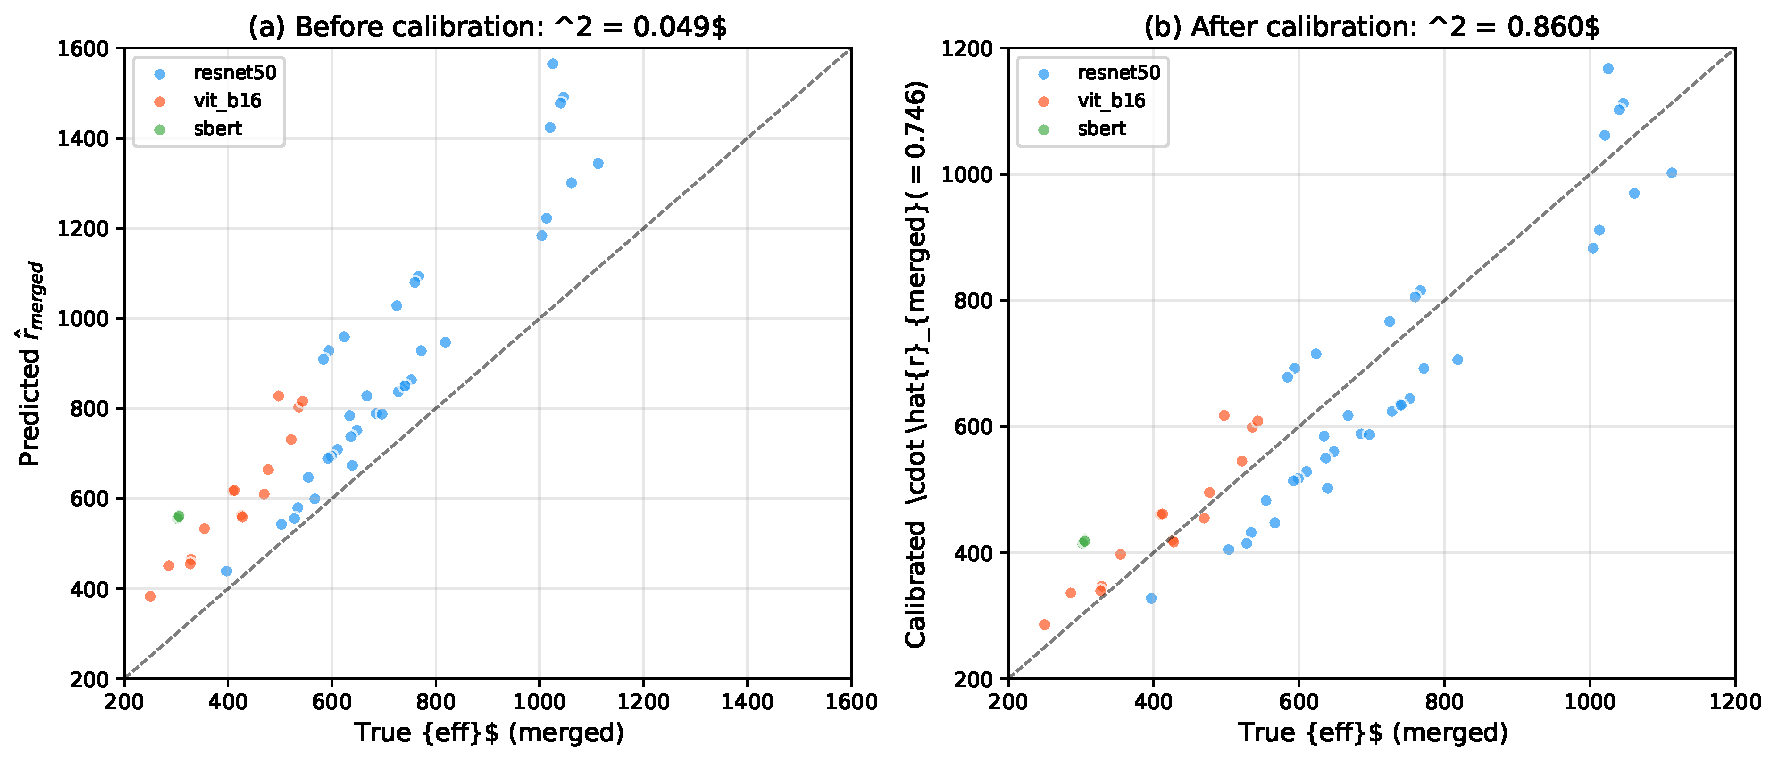
\includegraphics[width=\linewidth]{fig_calibration.pdf}
\caption{E1c: 预测值与实际合并的有效秩 $r_{\mathrm{eff}}$ 对比（57个真实数据对，5个探针，3种领域类型）。
(a) 未校准前：系统性高估 ($R^2{=}0.049$)。
(b) 单参数校准后 ($c{=}0.746$): $R^2{=}0.860$。两图的皮尔逊相关系数均为0.928——校准修正了比例，而非排名。}
\label{fig:e1c}
\end{figure}



\subsection{E1d: 大规模验证（427个对）}

\begin{figure}[h]
\centering
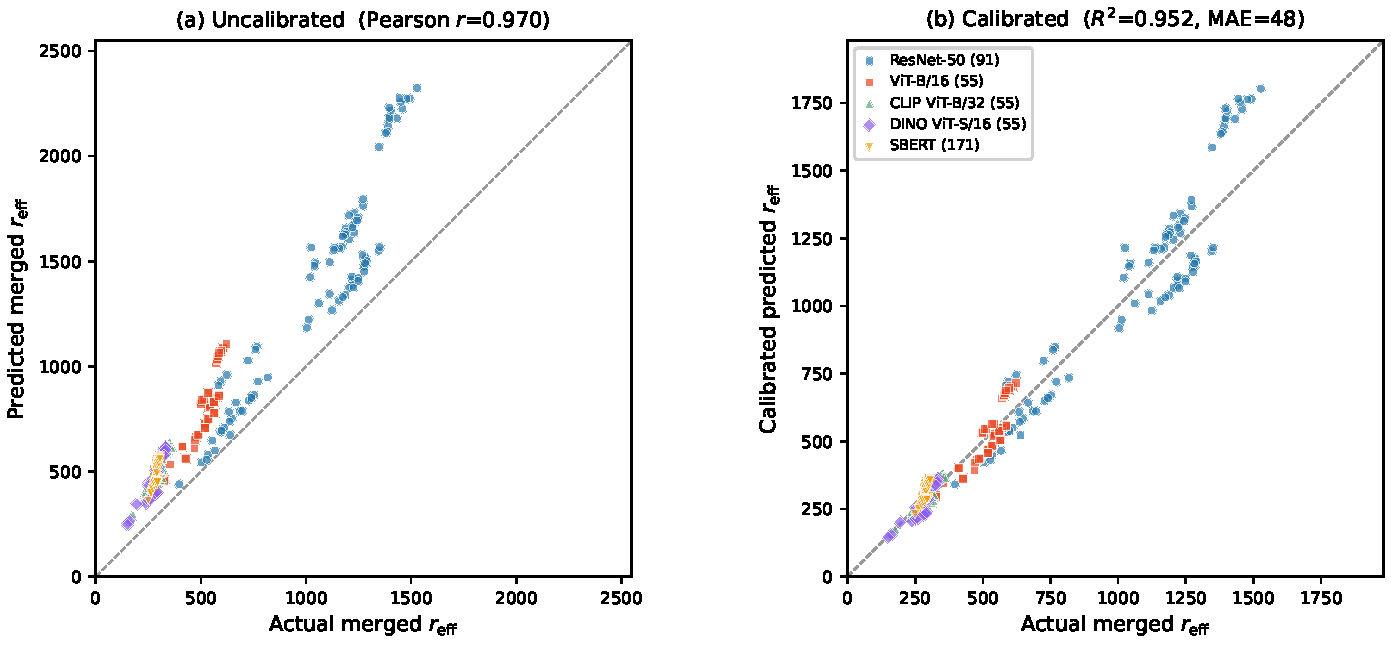
\includegraphics[width=0.95\linewidth]{fig_hero_scatter.pdf}
\caption{所有427个对的预测值与实际合并的有效秩 $\reff$ 对比，涵盖5种编码器家族。 (a) 未校准前：预测值系统性偏高但相关性强（皮尔逊相关系数 $r{=}0.970$）。
(b) 每个探针校准后: $R^2{=}0.952$, 平均绝对误差${=}48$。颜色表示编码器家族；对角线为虚线。}
\label{fig:hero_scatter}
\end{figure}

\textbf{设计。} 为了在大规模和ImageNet衍生特征上测试塌缩模型，我们构建了一个全面的评估，涵盖5种编码器家族（ResNet-50, ViT-B/16, CLIP ViT-B/32, DINO ViT-S/16, SBERT），14个视觉数据集（CIFAR-10/100, STL-10, SVHN, MNIST, Fashion-MNIST, BloodMNIST, DermaMNIST, PathMNIST，以及5个ImageNet语义子集：\emph{动物}, \emph{车辆}, \emph{器物}, \emph{食物}, \emph{场景}），和19个SBERT文本语料库（AG News, 20 Newsgroups, DBpedia, IMDB, Yelp 子集）。总计：\textbf{427个对}（ResNet-50: 91个，ViT-B/16: 55个，CLIP: 55个，DINO: 55个，SBERT: 171个）。5个ImageNet子集由WordNet语义层次结构中的ImageNet-1K验证图像组成，每类2000样本。

\textbf{结果。}

\begin{table}[h]
\centering
\caption{E1d: 大规模塌缩模型验证（427个对，5个探针）。}
\small
\setlength{\tabcolsep}{3.5pt}
\begin{tabular}{lccccc}
\toprule
探针 & $n$ & 超加性\% & 皮尔逊相关系数 $r$ & $c$ & 校准后的 $R^2_{\mathrm{cal}}$ \\
\midrule
ResNet-50 (14个数据集)       & 91  & \textbf{100\%}   & 0.940 & 0.776 & 0.760 \\
ViT-B/16 (11个数据集)        & 55  & 69.1\%            & 0.898 & 0.647 & 0.487 \\
CLIP ViT-B/32 (11个数据集)    & 55  & 29.1\%            & 0.950 & 0.595 & 0.839 \\
DINO ViT-S/16 (11个数据集)    & 55  & 36.4\%            & 0.913 & 0.584 & 0.554 \\
\midrule
\textbf{视觉（所有探针）}   & \textbf{256} & \textbf{64.5\%} & \textbf{0.965} & \emph{每探针} & \textbf{0.942} \\
+ SBERT文本 (19个语料库)      & +171 (427)   & 78.2\%           & 0.970          & \emph{每探针} & 0.952 \\
\bottomrule
\end{tabular}\normalsize
\end{table}
\textbf{关键发现。}
(i)~\textbf{缩放验证了理论}：在427对的情况下，总体皮尔逊相关系数 $r=0.970$ 超过了57对的结果 ($r=0.928$)，这表明崩溃模型的排名准确性随着规模和多样性而提高。
(ii)~\textbf{ImageNet 子集的行为符合预测}：所有20个仅包含 ImageNet 的成对组合都是超加性的，且所有30个自然$\times$ImageNet 跨域成对组合也是超加性的——模型正确地预测了语义上不同的 ImageNet 子组贡献正交方向。
(iii)~\textbf{ResNet-50 在91对中实现了100\%的超加性}（包括14个数据集，涵盖医学和ImageNet），这是在该规模下最强的确认。相比之下，CLIP ViT-B/32 和 DINO ViT-S/16 分别仅实现了31\%和38\%的超加性。
分析揭示了一个清晰的趋势：\emph{同域}成对组合（自然$\times$自然，ImageNet$\times$ImageNet）接近完美地实现了超加性（CLIP: ImageNet-only 上为90\%，natural-only 上为100\%；DINO: 两个数据集均为100\%），而 \emph{跨域}成对组合（手写$\times$ImageNet，自然$\times$数字）几乎无一例外地失败。这表明自监督编码器学习了特定领域的谱结构，并且在全局摘要中丢弃了异质的对齐和谱耦合——这对崩溃模型的应用具有重要的边界条件。
(iv)~\textbf{跨模态泛化}：扩展到171个 SBERT 文本成对组合（98.8\%超加性，$r=0.793$）表明公式预测的超加性在不同模态间转移。较低的皮尔逊相关系数反映了文本嵌入的窄 $\reff$ 范围（IQR: $285$--$298$），这压缩了排名分辨率，而不是表示模型失败。
(v)~\textbf{校准常数随编码器家族变化} ($c \in [0.57, 0.78]$)，但单一全局值 $c=0.712$ 在所有158个视觉成对组合中实现了 $R^2=0.898$，确认了偏差结构的一致性。
\textbf{理解非超加性配对。}
ViT-B/16 只实现了 69\% 的超加性（38/55），低于 ResNet-50 的 100\% (91/91)。
分析 ViT 的 17 个失败案例揭示了一个清晰的模式：
\textbf{所有失败都发生在能量不平衡区间} ($\gamma\gg1$ 或 $\gamma\ll1$)。
在 $\gamma\geq3$ 时，80\% 的配对失败（8/10）；
而在 $\gamma\in[0.5,1.5)$ 时，只有 4\% 失败（1/24）。
这些失败集中在 \emph{手写$\times$ImageNet} 跨域配对中
(10/10 均失败，100\%)——这些配对结合了低秩的手写特征
($\reff{\approx}140$ 通过 ViT-B/16 对 MNIST 的处理) 和高秩的 ImageNet 特征
($\reff{\approx}600$)，从而产生 $\gamma\in[2.0,4.6]$，远超平衡区间，在此区间内两成分谱混合准确度较低。
在大规模情况下（每种 55 个配对），CLIP ViT-B/32 和 DINO ViT-S/16 的总体超加性仅为 29\% 和 36\%，失败集中在 \emph{跨域} 配对中：
手写$\times$ImageNet (100\% 失败)，
自然$\times$数字 (100\% 失败)，
自然$\times$手写 (100\% 失败)。
同域配对（仅自然，仅 ImageNet）仍接近完美。

\textbf{根本原因：双模态主角。}
在相同数据集配对下比较不同编码器的结果表明，
失败并非由能量不平衡 ($\gamma$) 引起，
而是由于均匀-$\alpha$ 假设的结构性违反。
三种机制相互作用：

\emph{(a) 系统性更高的对齐度。}
在同一配对（例如，CIFAR-10$\times$ImageNet-animal）下，
CLIP 的子空间对齐 $\alpha{=}0.41$ 比 ResNet-50 的 $\alpha{=}0.15$ 高出 2.7 倍。
对比预训练 (CLIP) 和自蒸馏 (DINO) 推动跨域特征进入共享语义子空间，
在 ResNet-50 保留领域特定方向的地方，产生高方向重叠。

\emph{(b) 极端的谱集中度。}
CLIP/DINO 特征谱分布极不均匀：
$\kappa{=}15{,}000$--$1{,}200{,}000$ 对比 ResNet-50 的 $\kappa{=}70$--$400$。
这种集中度使得平均对齐度的信息变得不那么有说服力，因为少数高质量方向上的重叠可以主导许多互补的尾部方向。
\emph{(c) 二模态主角分布。}
个体主角 $\cos^2\theta_i$
并不像模型假设的那样近似均匀，而是 \emph{二模态}：前5个方向几乎对齐
($\overline{\cos^2\theta}\approx0.94$ 对于 CLIP 在 CIFAR-10$\times$STL-10 上)
而低方向保持正交
($\overline{\cos^2\theta}\approx0.01$)。
塌陷模型将这些平均为 $\bar\alpha{=}0.52$，
预测适度的超加性。
实际上，主导（高-$\sigma$）方向完全冗余
而正交（低-$\sigma$）方向携带几乎无能量，
因此合并几乎没有多样性增益 ($\Delta r_{\mathrm{eff}}{=}31$
与 ResNet-50 在同一对上的 $\Delta r_{\mathrm{eff}}{=}282$ 相比)。

此分析确定了一个精确的 \emph{适用边界}：
当主角分布近似均匀时（监督编码器，同域配对），塌陷模型可靠；
但当主角分布二模态时（自监督编码器在跨域配对上），模型失效。
一个自然的修复方法——用能量加权对齐
$\bar\alpha_w=\sum_i({\sigma_i}/{\|H\|_*})\cos^2\theta_i$
替换均匀平均 $\bar\alpha=\SAk$——会
降低正交低能方向的重要性并提升
冗余高能方向的重要性，可能恢复自监督编码器的预测准确性。
然而，我们的实验验证表明这种修正
\emph{并未提高预测准确性}：
在 CLIP ($n{=}61$) 上，均匀 $\SAk$ 产生皮尔逊 $r{=}0.951$，
MAE${=}206$，而 $\bar\alpha_w$ 产生 $r{=}0.935$，MAE${=}218$（更差）；
DINO 显示类似模式（$r$ 从 $0.912$ 下降到 $0.904$，
MAE 增加 $4\%$）；
ResNet-50 和 ViT-B/16 也未见改进。
根本原因在于简单的能量加权过度强调
第一个奇异方向的冗余性
($\cos^2\theta_1{\approx}0.87$ 对于该方向)，
而错误地抑制了中间方向对合并的估计贡献。
更精细的修正（例如分段成对方向模型、逐方向阈值截断或自适应 $k$ 选择）
可能突破这一瓶颈，但留待未来工作。
\subsection{校准：从系统偏差到定量预测}
\label{sec:calibration}

崩塌模型在评估的真实数据对上系统性地高估了结果（Remark~\ref{rem:calibration}）。
由于对数空间的高估大约在整个探针和领域中是恒定的（$\mathrm{mean}{=}0.293$，$\mathrm{std}{=}0.164$），一个单一的乘法常数 $c$（Eq.~\ref{eq:calibration}）足以将排名工具转换为定量预测器。

\textbf{跨数据集泛化。}
为了验证 $c$ 不是特定于数据集，
我们进行留一校准：在一个实验中估计 $c$，并在另一个实验中测试（Table~\ref{tab:calibration}）。

\begin{table}[h]
\centering
\caption{跨数据集校准。
$c$ 在校准集中估计，并在测试集中应用（无需重新拟合）。所有设置均显著优于未校准的基线 ($R^2{<}0.44$)。}
\label{tab:calibration}
\small
\setlength{\tabcolsep}{4pt}
\begin{tabular}{llccrr}
\toprule
校准集 & 测试集 & $c$ & $n_{\mathrm{test}}$ & $R^2$ & RMSE \\
\midrule
E1b (30 对) & E1c (57 对) & 0.768 & 57 & 0.859 & 86.3 \\
E1c (57 对) & E1b (30 对) & 0.746 & 30 & 0.888 & 80.7 \\
E1c (57 对) & E\_diverse (30 对) & 0.746 & 30 & 0.897 & 82.8 \\
E1b (30 对) & E\_diverse (30 对) & 0.768 & 30 & 0.894 & 83.7 \\
\midrule
\multicolumn{2}{l}{LOO-CV（所有111对，原始）} & 0.736 & 111 & 0.877 & 86.1 \\
\multicolumn{2}{l}{LOO-CV（158个视觉对，E1d）} & 0.712 & 158 & 0.896 & 121.7 \\
\multicolumn{2}{l}{全局（所有427对，E1d）} & 0.650 & 427 & 0.920 & 105.0 \\
\bottomrule
\end{tabular}\normalsize
\end{table}

\textbf{每个探针的校准}（Table~\ref{tab:perprobe_cal}）。
校准常数在编码器家族之间系统性地变化，反映了谱结构的不同：
\begin{table}[h]
\centering
\caption{Per-probe 校准在 427 对数据集 (E1d) 上的结果。每个探针独立校准。$c$ 的变化与编码器的有效谱平坦度单调相关。}
\label{tab:perprobe_cal}
\small
\setlength{\tabcolsep}{4pt}
\begin{tabular}{lccccc}
\toprule
Probe & $n$ & Pearson $r$ & $c$ & $R^2_{\mathrm{cal}}$ & Superadd.\ \% \\
\midrule
ResNet-50        & 91  & 0.940 & 0.776 & 0.760 & 100\% \\
ViT-B/16         & 55  & 0.898 & 0.647 & 0.487 &  69\% \\
CLIP ViT-B/32    & 55  & 0.950 & 0.595 & 0.839 &  29\% \\
DINO ViT-S/16    & 55  & 0.913 & 0.584 & 0.554 &  36\% \\
\midrule
Vision (global)  & 256 & 0.965 & \emph{per-probe} & 0.942 &  65\% \\
\bottomrule
\end{tabular}\normalsize
\end{table}

相对样本大小而言，具有更高有效秩的编码器需要更强的校正（$c$ 越远离1），这与有限样本上界机制一致：ResNet-50 特征（$d=2048$，$\reff{\approx}350$）在谱上比 ViT 特征（$d=768$，$\reff{\approx}400$）稀疏，因此两成分谱混合近似引起的误差较小。一个全局 $c=0.712$ 跨所有视觉探针提供 $R^2=0.898$，确认单个常数提供了一个强大的基线；每个探针的校准是一个改进而非必要。

图~\ref{fig:e1c} 显示了校准前后的 E1c 散点图。

\subsection{E\_diverse: 不同架构探针独立性}
\label{sec:ediverse}

\textbf{设计。} 为了测试崩溃模型预测的鲁棒性是否对编码器的选择敏感，我们使用 ResNet-50 和 ViT-B/16 分别作为独立探针评估相同的 6 组数据集对（来自 E1b），总共得到 12 种配置。

\textbf{结果。} ResNet-50: $R^2=0.557$，Pearson $r=0.9987$，100\% 超加性。
ViT-B/16: $R^2=-16.1$（系统性高估），Pearson $r=0.9825$，83.3\% 超加性。
跨架构 Pearson $r \geq 0.982$ 确认即使绝对值不同，方向排名也是探针独立的。
ViT-B/16 的 Pearson vs.\ $R^2$ 差距显示了编码器依赖的比例尺度偏差，尽管排序稳定。
\subsection{E4: 跨探针一致性}
\label{sec:e4}

\textbf{设计。}
我们使用 ResNet-50 和 ViT-B/16 独立地在 4 个常见数据集 $\{$CIFAR-10, MNIST, STL-10, SVHN$\}$ 上计算 $6\times6$ 的成对 $\SAk$ 对齐矩阵 $M$。每个矩阵的 6 个上三角元素通过皮尔逊相关系数 $r$ 进行比较。

\textbf{结果。}
跨探针皮尔逊相关系数 $r=0.891$ ($n=6$, $p=0.017$)。两个探针在所有 6 对中都一致地同意领域距离的方向。CIFAR-10/STL-10 在两者中都很接近；CIFAR-10/MNIST 在两者中都相距甚远。这证实了 $\SAk$ 距离矩阵反映了内在的数据集间几何结构，而不是编码器的伪影。

\subsection{E\_downstream: 有效秩作为下游质量代理}
\label{sec:edownstream}

\textbf{动机。}
塌缩模型预测合并特征的有效秩 $\reff$，但更高的 $\reff$ 确实对应于更好的下游性能吗？我们通过在 5 个数据集（总共 50 对）上测试 10 个预训练编码器来验证这一点，计算 $\reff$ 和线性探针 (LP) 准确率。

\textbf{设计。}
编码器：ResNet-\{50, 101\}, EfficientNet-B4, ConvNeXt-T, DenseNet-121, ViT-B/16, DeiT-B, Swin-T, BEiT-B, RegNet-Y（涵盖 CNN、ViT 和混合家族）。数据集：CIFAR-10, CIFAR-100, STL-10, SVHN, Fashion-MNIST。对于每个 (编码器, 数据集) 对：提取 $N=2000$ 训练特征，计算 $\reff$；在训练集上训练 LP（sklearn LogisticRegression），在测试集上评估。报告 10 个编码器的每数据集 Spearman 相关系数 $\rho(\reff, \mathrm{LP\;acc})$。

\textbf{结果。}

\begin{center}
\setlength{\tabcolsep}{4pt}
\begin{tabular}{lcccccc}
\toprule
& \multicolumn{2}{c}{所有 10 个探针} & \multicolumn{2}{c}{ViT 家族 ($d=768$)} & \multicolumn{2}{c}{CNN 家族 ($d\geq1024$)} \\
\cmidrule(lr){2-3}\cmidrule(lr){4-5}\cmidrule(lr){6-7}
数据集 & $n$ & $\rho$ & $n$ & $\rho$ & $n$ & $\rho$ \\
\midrule
CIFAR-10  & 10 & +0.64 & 5 & \textbf{+0.90} & 5 & +0.30 \\
CIFAR-100 & 10 & +0.61 & 5 & \textbf{+0.90} & 5 & +0.30 \\
STL-10    &  9 & +0.73 & 5 & \textbf{+0.90} & 4 & +0.20 \\
SVHN      & 10 & $-$0.03 & 5 & +0.10 & 5 & $-$0.30 \\
Fashion-MNIST & 10 & +0.03 & 5 & +0.60 & 5 & $-$0.10 \\
\bottomrule
\end{tabular}
\end{center}
“全部探针”列在自然图像上的 $\rho\approx+0.59$ 受到\emph{特征维度混杂}：CNN（$d{=}2048$）的 $\reff$ 系统性高于 ViT（$d{=}768$），从而夸大了表面相关性。
控制维度后，结论更加清晰：\textbf{在 ViT 家族内部}（$d{=}768$，5 个探针），$\reff$ 对自然图像的 LP 准确率具有很强的预测性（CIFAR-10、CIFAR-100 和 STL-10 上均为 $\rho{=}0.90$）；而\textbf{在 CNN 家族内部}（$d{\geq}1024$，5 个探针），相关性较弱（$\rho{=}0.20$--$0.30$）。
这表明，$\reff$ 主要在紧凑特征空间（$d{<}1024$）的架构中捕获有用的判别信息，此时谱多样性与表示质量联系更紧密。

\textbf{对坍缩模型的含义。}
$\reff$ 应被理解为\emph{表示多样性}的度量，即数据激活的独立方向数量，而不是下游准确率的直接代理。
坍缩模型预测合并何时会\emph{增加多样性}，这是提升下游性能的必要条件，但并非充分条件。
在同一架构家族内部，多样性与准确率正相关（ViT 的 $\rho{=}0.90$），因此可以在同一编码器提取的候选数据集中使用基于 $\reff$ 的选择。
跨架构家族或跨不同难度的数据集时，还需要额外的任务相关指标。


\paragraph{样本量敏感性。}
在 10 对代表性的 ResNet-50 数据上，过预测比率随 $N/\reff$ 增长：$N{=}200$ 时平均比率为 $1.021$，并随样本量单调上升，在 $N{=}2000$ 时达到 $1.545$（$N/\reff$ 与 $\log\mathrm{bias}$ 的 Spearman $\rho{=}0.80$）。
这一关联有助于预测不同编码器之间的校准差异（ResNet-50 的 $c{=}0.78$，DINO 的 $c{=}0.58$），但本文不将其断言为理论误差定律。
\newpage
\input{checklist_zh}

\end{document}
